%%%%%%%%%%%%%%%%%%%%%%%%%%%%%%%%%%%%%%%%%%%%%%%%%%%%%%%%%%%%%%%%%%%%%%%%%%

\chapter{アクセス環境の影響の調査}
\label{chap:access}
本章では,アクセス環境による通信品質の影響を調査する.アクセス環境とは,クライアントの端末からサーバーまでの経路上の回線の種別や通信方式などのことを指す.本研究では,インターネットサービスプロバイダ(ISP)の網,アクセス網の種類,インターネット接続方式の3つをアクセス環境として分類する.
\section{調査方法}
調査にはiNonius Speed Test\cite{iNonius}の計測ログを用いる.iNonius Speed Testの測はWebブラウザを利用してIPv4/IPv6デュアルスタック環境におけるインターネット通信品質を計測できるサービスである.HTTP通信による計測を実現しているLibrespeed\cite{librespeed}を利用して計測を行っている.計測区間は\cref{fig:Measurment}のようにユーザー端末から計測サイトまでの区間である.
計測ログには\cref{tab:loginfo}の情報が含まれている.データの計測期間は 2022 年 10 月 1 日〜 2023 年 5 月 31 日と 2023 年 6 月 1 日 〜 2024 年 6 月 31 日のログを使用した.前者の期間を(1)とし,後者の期間を(2)とする.これらのログのうち,IPv4/IPv6 デュアルスタック環境における計測結果を分析の対象とした.デュアルスタック環境からの計測の判定はuseridを基に行った.useridは計測ごとにユーザーに割り当てられる.デュアルスタック環境からの計測の場合,IPv4 と IPv6 の計測結果がそれぞれに同じuseridで記録される.シングルスタック環境からの計測の場合は,計測ログ内に同じuseridが存在しないため,それらを除外することでデュアルスタック環境の計測結果のみを抽出した.また,外れ値として計測が未完了な項目を1つでも含むデータは除外した.

%\begin{comment}
\begin{figure}[htbp]
    \centering
    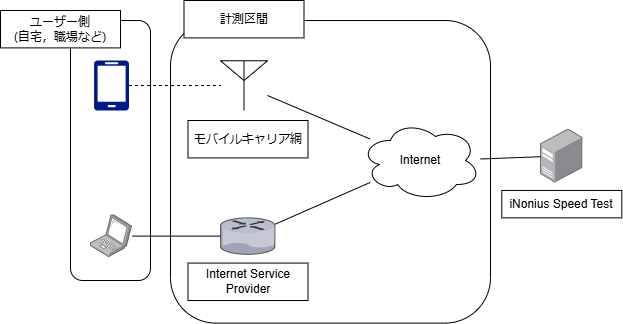
\includegraphics[width=1.0\textwidth]{fig/Measurment.png}
    \caption{iNonius Speed Testの計測区間}
    \label{fig:Measurment}
\end{figure}
\FloatBarrier
\begin{table}[htbp]
    \caption{iNonius スピードテストの計測ログの情報}
    \label{tab:loginfo}
    \begin{center}
        \begin{tabular}{cc} \hline
            項目 & 説明 \\ \hline \hline
            userid & ユーザーを識別するID \\
            id & 計測ログを識別するID \\
            timestamp & 計測が行われた日時 \\
            ip & 計測元のIPアドレス \\
            isIpv4 & IPv4で計測されたかどうかのフラグ \\
            ispInfo & ISPに関する情報(社名,本拠地など) \\
            ua & 計測端末のOSやブラウザの情報 \\
            connectionType & Network Information APIの結果 \\
            lang & ブラウザの言語設定 \\
            dl & ダウロードのスループットの計測結果[Mbps] \\
            ul & アップロードのスループットの計測結果[Mbps] \\
            ping & RTTの計測結果[ms] \\
            jitter & RTTの揺らぎの計測結果[ms] \\
            mss & MSSのサイズ \\
            ttl & TTLの値 \\
            lossRate & パケットロス率の計測結果[\%] \\
            defaultIp & デフォルトのIP \\
            srcPort & 計測元のソースポート \\ \hline
        \end{tabular}
    \end{center}
\end{table}
\FloatBarrier
%\end{comment}

\section{アクセス環境の判定}
\label{label:accesstype}
アクセス環境は\cref{tab:accesstype} のように分類する.ISPの網の判定には,計測ログのispInfoを使用する.この値はLiberSpeedが,計測の過程でipifo.io\cite{ipinfo}に計測元のIPアドレスの情報を問い合わせて取得した情報である.IPv4/IPv6のそれぞれの計測結果に含まれるこの値を比較して判定した.

アクセス網の種類の計測ログに含まれる情報だけでは判断できないため,GeoLocation Technology が提供する「どこどこ JP」\cite{docodoco}を使用した.このサービスは.IPアドレスに地理情報や企業情報などを紐づけたデータベースで,今回使用したアクセス網の種類の判定なども含まれる.計測ログのIPアドレスを基に,このサービスを用いてアクセス網の種類を判定した.


インターネット接続方式の判定には,先行研究で用いられているMSSの値を用いた判定方法を使用した.判定の基準は\cref{tab:mss}の通りである.この表をもとに,IPv4/IPv6のそれぞれの計測結果に含まれるMSSの値でIPoEかPPPoEかを判定し,最後に組み合わせてインターネット接続方式を判定した.

%\begin{comment}
\begin{table}[htbp]
    \caption{アクセス環境の分類}
    \label{tab:accesstype}
    \begin{center}
        \begin{tabular}{cc} \hline
            アクセス環境の分類 & 詳細な分類 \\ \hline \hline
            \multirow{2}{*}{ISPの網} & IPv4/IPv6で同じ場合 \\
            & IPv4/IPv6で異なる場合 \\
            \hline
            \multirow{3}{*}{アクセス網の種類} & FTTH \\ 
            & CATV \\
            & Mobile \\
            \hline
            \multirow{3}{*}{インターネット接続方式} & IPv4/IPv6共にIPoE \\
            & IPv4/IPv6共にPPPoE \\
            & IPv4がPPPoE,IPv6がIPoE \\ \hline
        \end{tabular}
    \end{center}
\end{table}
\FloatBarrier
\begin{table}[htbp]
    \caption{インターネット接続方式の判定とMSSの値}
    \label{tab:mss}
    \begin{center}
        \begin{tabular}{cccc} \hline
            \multicolumn{2}{c}{インターネット接続方式}& \multicolumn{2}{c}{MSSのサイズ} \\
            IPv4& IPv6& IPv4& IPv6 \\ \hline \hline
            IPoE & IPoE & 1460 & 1440 \\
            PPPoE & PPPoE & 1452 & 1394 \\
            PPPoE & IPoE & 1452 & 1440 \\ \hline
        \end{tabular}
    \end{center}
\end{table}
\FloatBarrier
%\end{comment}

\section{スループットの調査}
\label{sec:throughput}
\cref{label:accesstype}で示したアクセス環境の違いによる集計結果を IPv4 と IPv6 のスループットの比較がわかるように\cref{fig:old_isp_dl}のように散布図とヒストグラムのグラフにして分析した.左下が IPv4 と IPv6 のスループットの相関を示す散布図で,左上と右下のヒストグラムがそれぞれ IPv4 と IPv6 のスループットの階級ごとの度数を表す.散布図の縦軸と右下のヒストグラムの縦軸,散布図の横軸と左上のヒストグラムの横軸はそれぞれ同じスケールになっている.

%%%%%%%%%%%%%%%%%%%%%%%%%%%%%%%%%%%%%%%%%%%%%%%%%%%%%%%%%%%%%%%%%%%%%%%%%%
\subsection{ISPの網によるスループットへの影響}
\label{subsec:isp_dl}
\cref{fig:old_isp_dl,fig:new_isp_dl} はそれぞれの期間のISPの網の違いによるダウンロードのスループットの比較を示す.ただし,ここで言う「ISPの網の違い」とはIPv4とIPv6で同じISPを使用した場合と異なるISPを使用した場合の2つを指す.\cref{fig:old_isp_dl} は(1)の期間の結果で,\cref{fig:new_isp_dl} は(2)の期間の結果である.\cref{old_sameISP_dl,new_sameISP_dl}は同じISPを使用した場合の結果で,\cref{old_diffISP_dl,new_diffISP_dl}は異なるISPを使用した場合の結果である.

\cref{old_sameISP_dl,old_diffISP_dl}を比較するとIPv4/IPv6のスループットの相関性に違いが見られる.これは\cref{fig:new_isp_dl}でも同様である.\cref{fig:old_isp_ul,fig:new_isp_ul}のそれぞれの(a)と(b)を比較すると,ダウンロードに比べて相関係数の値の差が小さいが概ね同様の傾向が見られる.
(b)の場合は,IPv4/IPv6で異なるISPであることから計測サーバーへの経路が異なる可能性があり,その結果IPv4/IPv6で相関性が低くなると考えられる.
そこで,ISPによってふるまいが異なる可能性があるのか確認するためにデータ数の多い3社に絞って分析を行う.ただし,データ数の都合上(2)の期間のみである.\cref{fig:new_isp_dl2,fig:new_isp_ul2}はそれぞれA社,B社,C社のISPの違いによるダウンロードとアップロードのスループットの比較を示す.3社ともそれぞれのIPv4/IPv6の間の相関性は高く,それぞれのヒストグラムの形も似ている.しかし異なるISP同士で比較すると,ヒストグラムのピークの現れる位置が異なることから,ISPによってふるまいが異なる可能性があることがわかる.

%\begin{comment}
\begin{figure}[htbp]
    \begin{center}
        \begin{subfigure}[b]{0.49\textwidth}
            \centering
            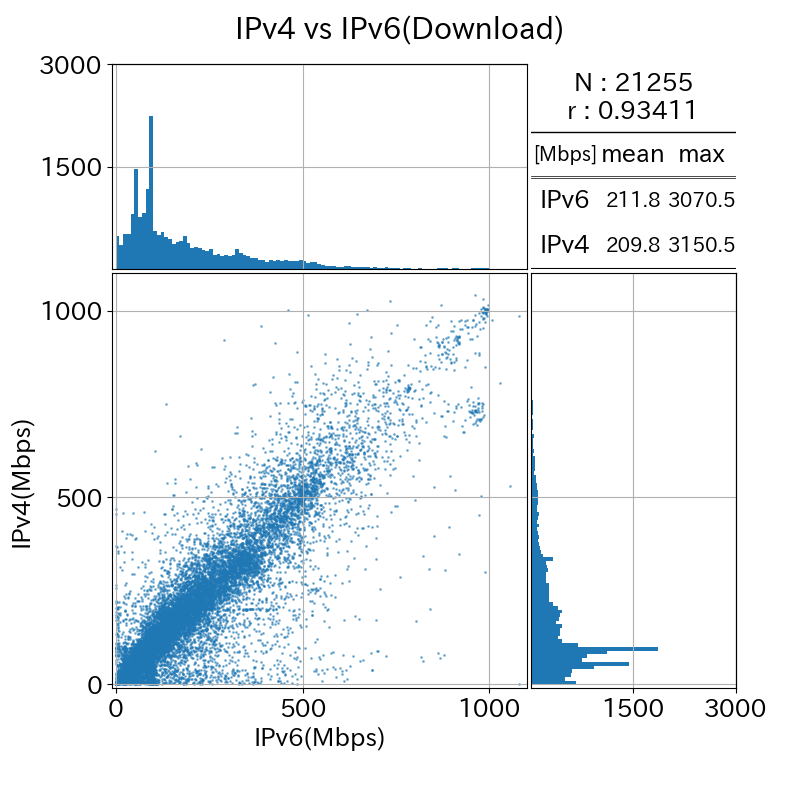
\includegraphics[width=1.0\textwidth]{fig/old_sameISP_dl.png}
            \subcaption{同じISPを使用した場合}
            \label{old_sameISP_dl}
        \end{subfigure}
        \begin{subfigure}[b]{0.49\textwidth}
            \centering
            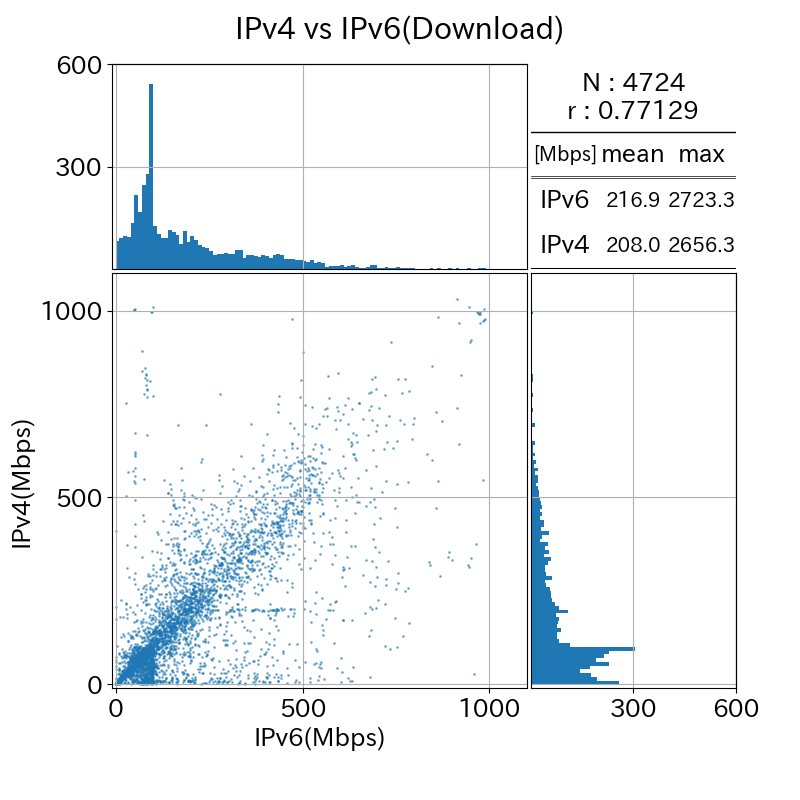
\includegraphics[width=1.0\textwidth]{fig/old_diffISP_dl.png}
            \subcaption{異なるISPを使用した場合}
            \label{old_diffISP_dl}
        \end{subfigure}
        \caption{(1)のダウンロードのスループット}
        \label{fig:old_isp_dl}
    
        \begin{subfigure}[b]{0.49\textwidth}
            \centering
            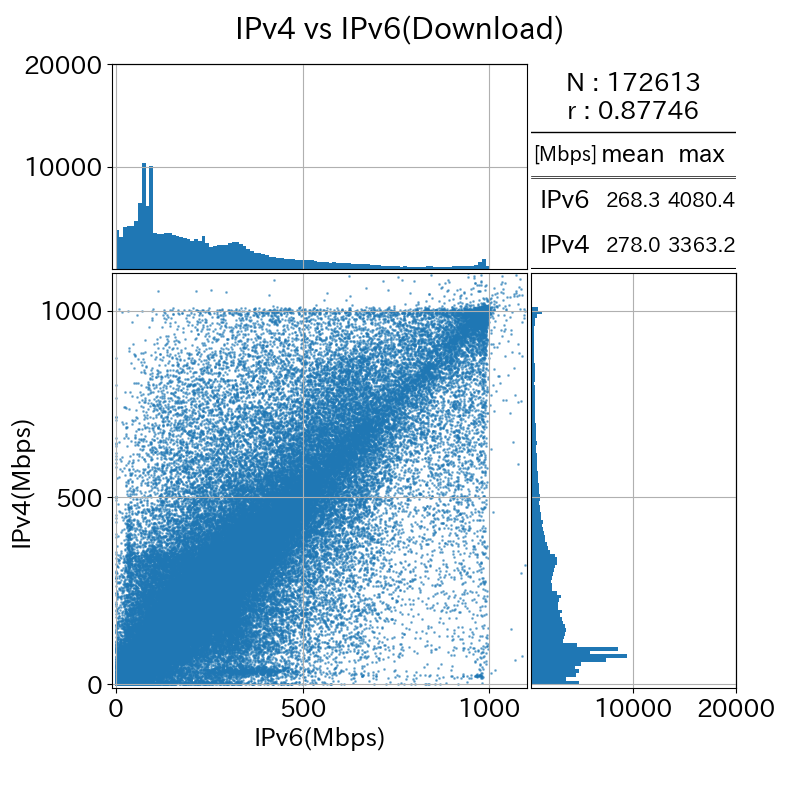
\includegraphics[width=1.0\textwidth]{fig/new_sameISP_dl.png}
            \subcaption{同じISPを使用した場合}
            \label{new_sameISP_dl}
        \end{subfigure}
        \begin{subfigure}[b]{0.49\textwidth}
            \centering
            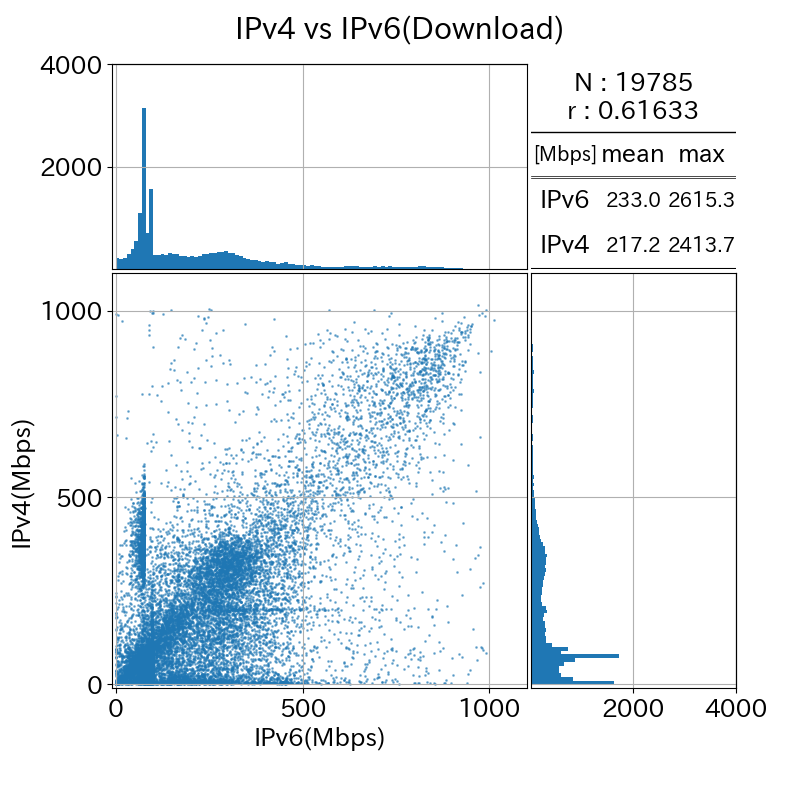
\includegraphics[width=1.0\textwidth]{fig/new_diffISP_dl.png}
            \subcaption{異なるISPを使用した場合}
            \label{new_diffISP_dl}
        \end{subfigure}
        \caption{(2)のダウンロードのスループット}
        \label{fig:new_isp_dl}
    \end{center}
\end{figure}
\FloatBarrier

\begin{figure}[htbp]
    \begin{center}
        \begin{subfigure}[b]{0.49\textwidth}
            \centering
            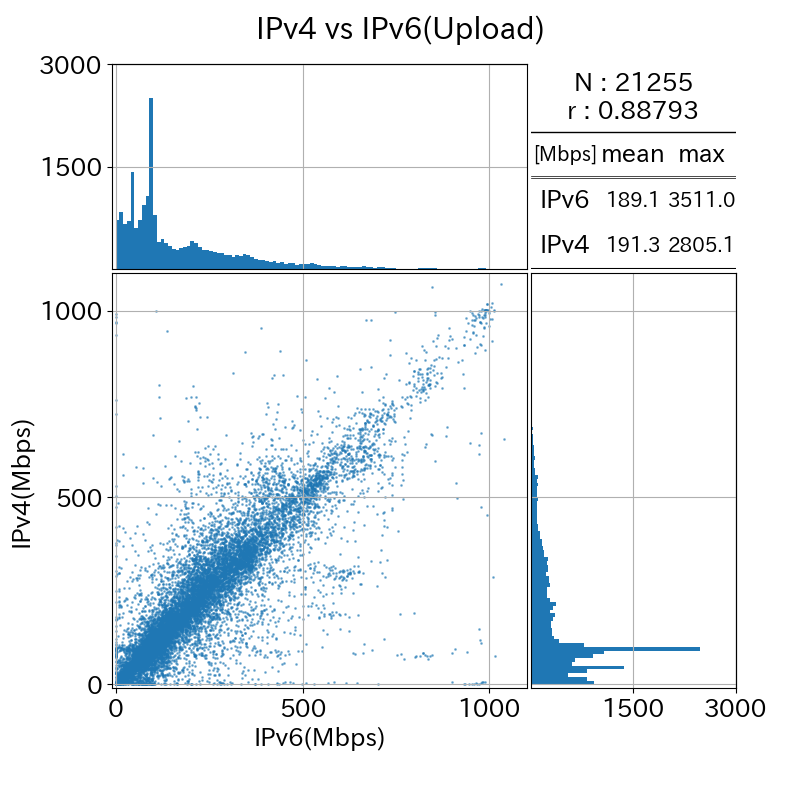
\includegraphics[width=1.0\textwidth]{fig/old_sameISP_ul.png}
            \subcaption{同じISPを使用した場合}
            \label{old_sameISP_ul}
        \end{subfigure}
        \begin{subfigure}[b]{0.49\textwidth}
            \centering
            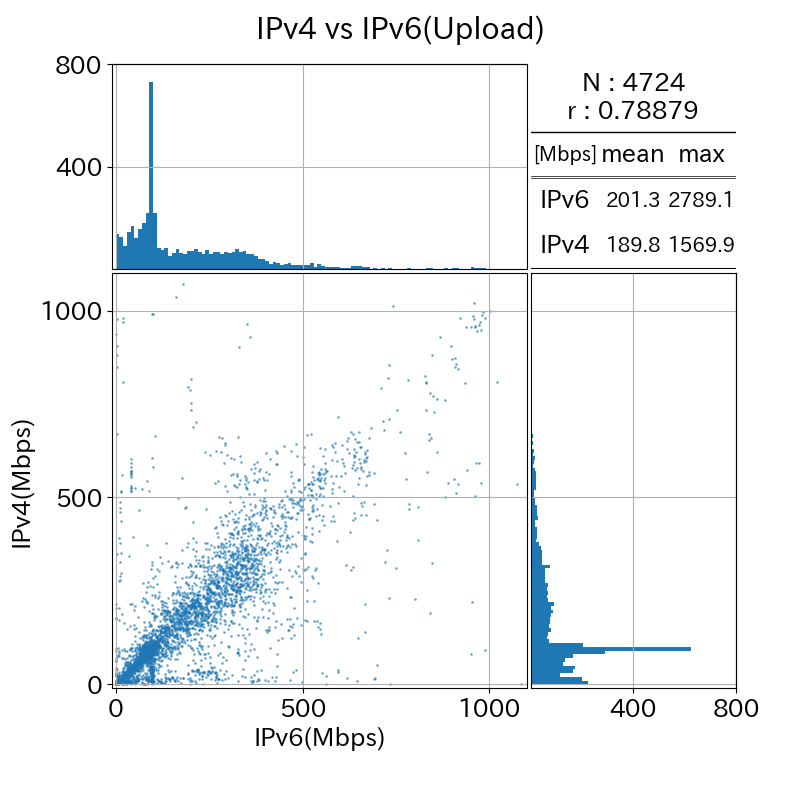
\includegraphics[width=1.0\textwidth]{fig/old_diffISP_ul.png}
            \subcaption{異なるISPを使用した場合}
            \label{old_diffISP_ul}
        \end{subfigure}
        \caption{(1)のアップロードのスループット}
        \label{fig:old_isp_ul}

        \begin{subfigure}[b]{0.49\textwidth}
            \centering
            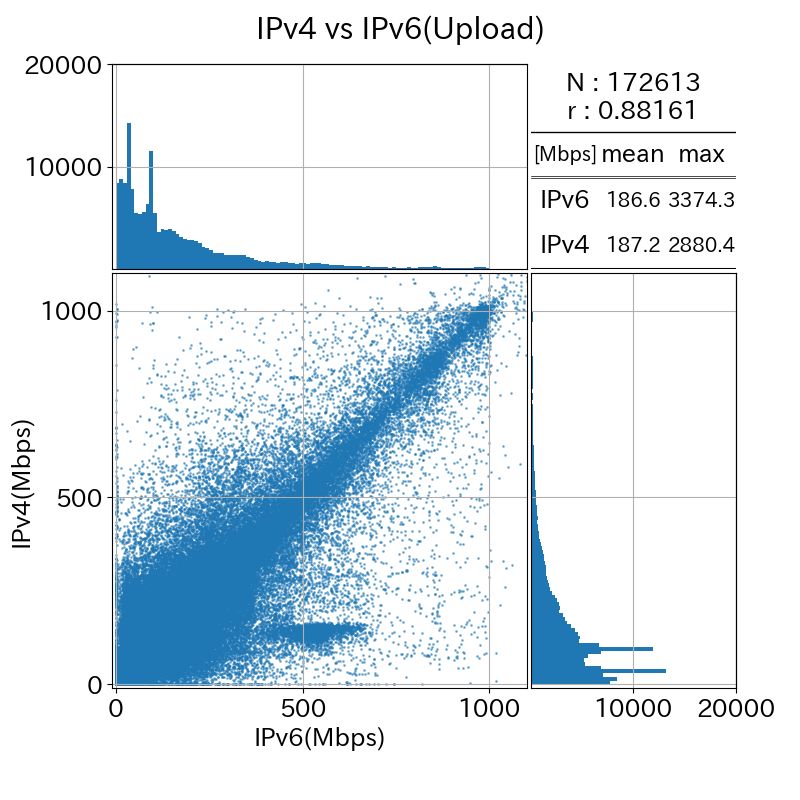
\includegraphics[width=1.0\textwidth]{fig/new_sameISP_ul.png}
            \subcaption{同じISPを使用した場合}
            \label{new_sameISP_ul}
        \end{subfigure}
        \begin{subfigure}[b]{0.49\textwidth}
            \centering
            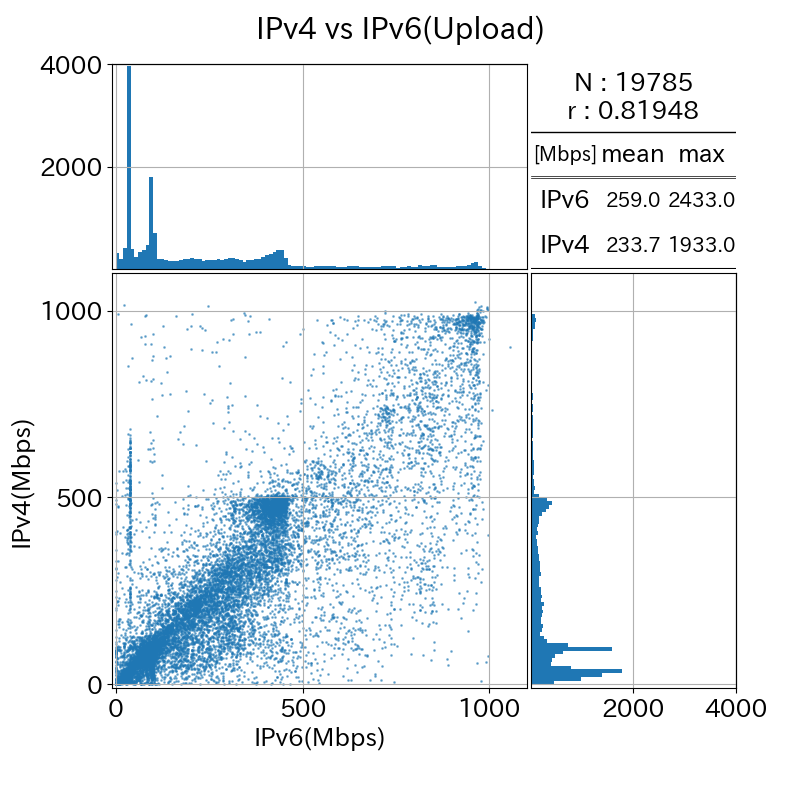
\includegraphics[width=1.0\textwidth]{fig/new_diffISP_ul.png}
            \subcaption{異なるISPを使用した場合}
            \label{new_diffISP_ul}
        \end{subfigure}
        \caption{(2)のアップロードのスループット}
        \label{fig:new_isp_ul}
    \end{center}
\end{figure}
\FloatBarrier

\begin{figure}[htbp]
    %\centering
    \begin{center}
        % 左側の図
        \begin{minipage}[t]{0.48\textwidth}
            \begin{center}
                \begin{subfigure}[b]{\textwidth}
                    \centering
                    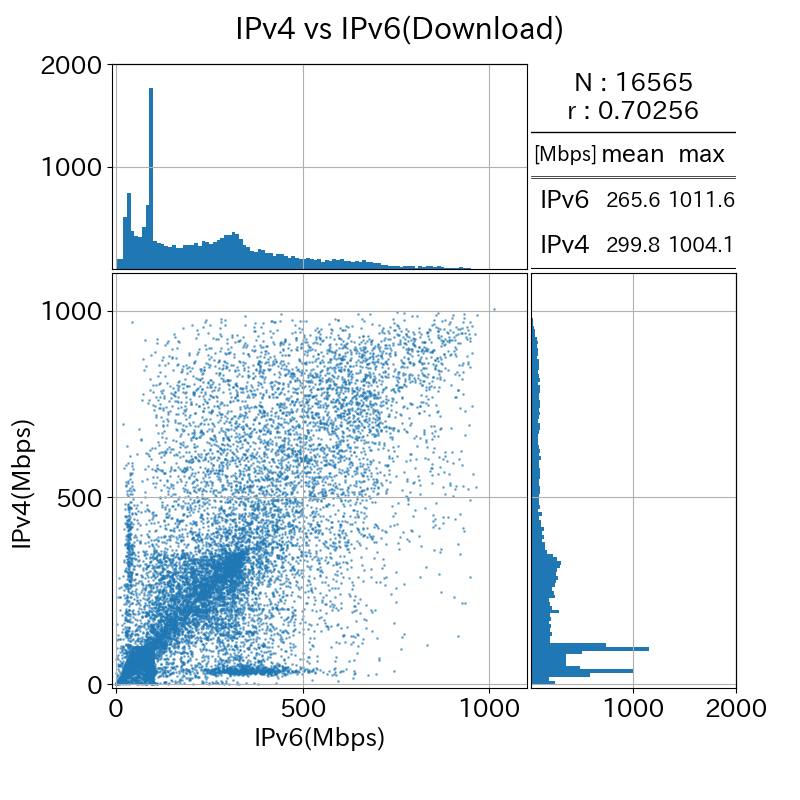
\includegraphics[width=0.85\textwidth]{fig/new_NTT_dl.png}
                    \subcaption{A社の場合}
                    \label{new_NTT_dl}
                    \end{subfigure}
                \begin{subfigure}[b]{\textwidth}
                    \centering
                    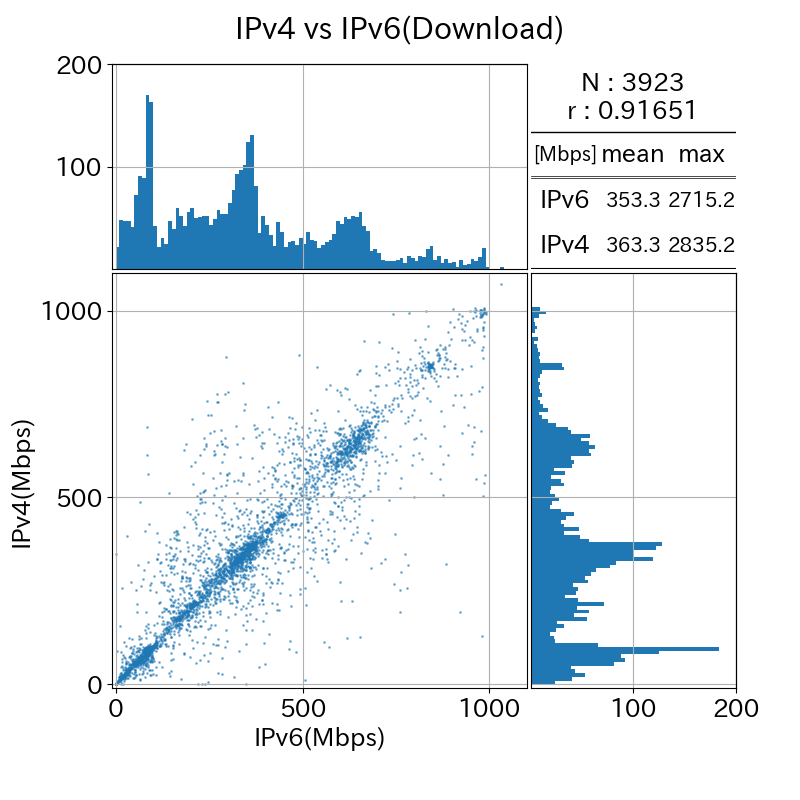
\includegraphics[width=0.85\textwidth]{fig/new_KDDI_dl.png}
                    \subcaption{B社の場合}
                    \label{new_KDDI_dl}
                \end{subfigure}
                \begin{subfigure}[b]{\textwidth}
                    \centering
                    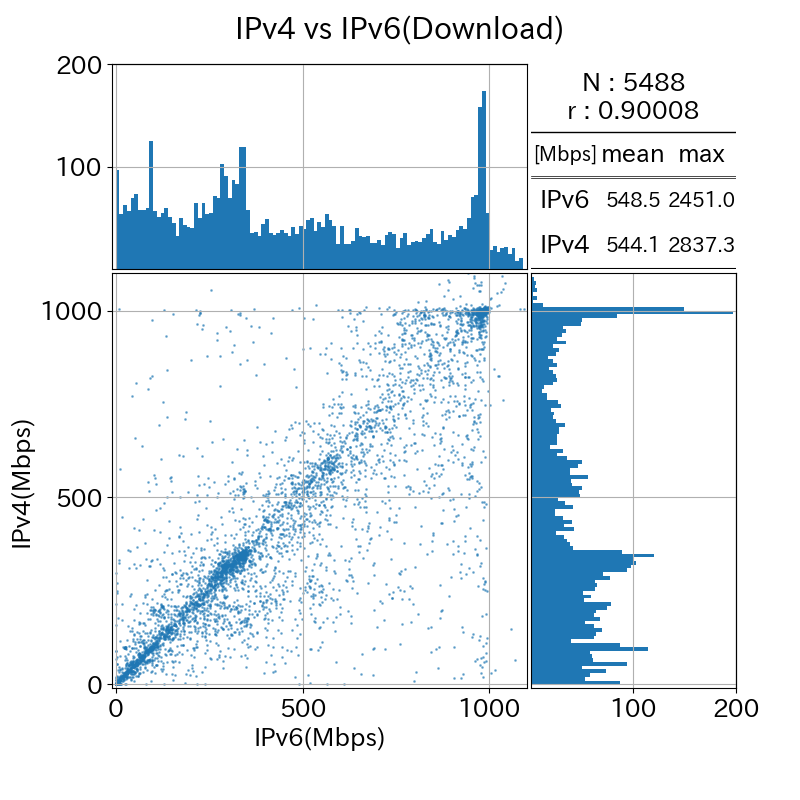
\includegraphics[width=0.85\textwidth]{fig/new_Sony_dl.png}
                    \subcaption{C社の場合}
                    \label{new_Sony_dl}
                \end{subfigure}
                \caption{ISPの違いによる\\ダウンロードのスループット}
                \label{fig:new_isp_dl2}
            \end{center}
        \end{minipage}
        \hfill
        % 右側の図
        \begin{minipage}[t]{0.48\textwidth}
            \begin{center}
                \begin{subfigure}[b]{\textwidth}
                    \centering
                    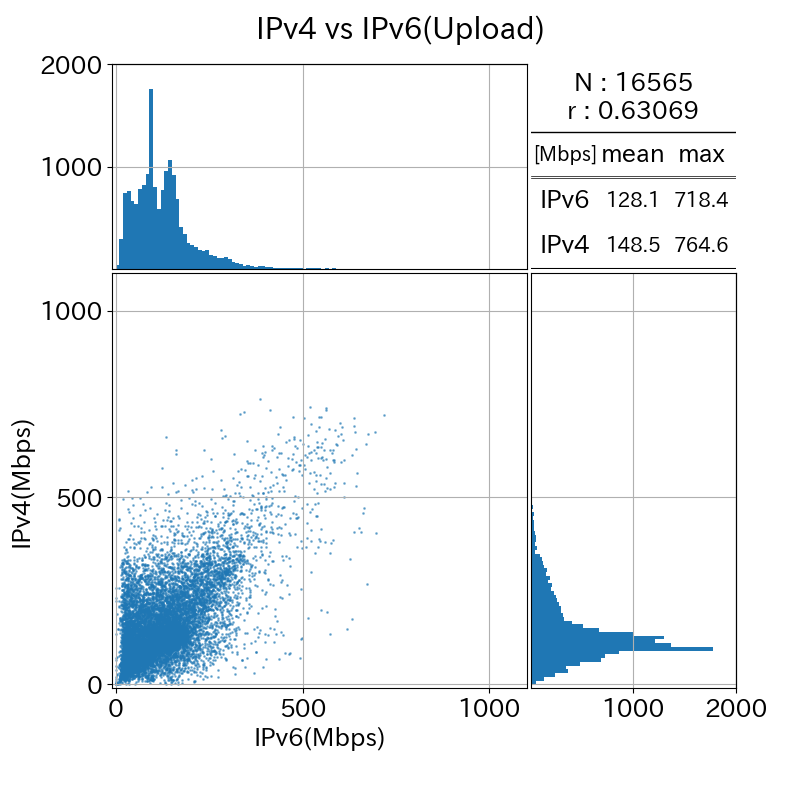
\includegraphics[width=0.85\textwidth]{fig/new_NTT_ul.png}
                    \subcaption{A社の場合}
                    \label{new_NTT_ul}
                \end{subfigure}
                \begin{subfigure}[b]{\textwidth}
                    \centering
                    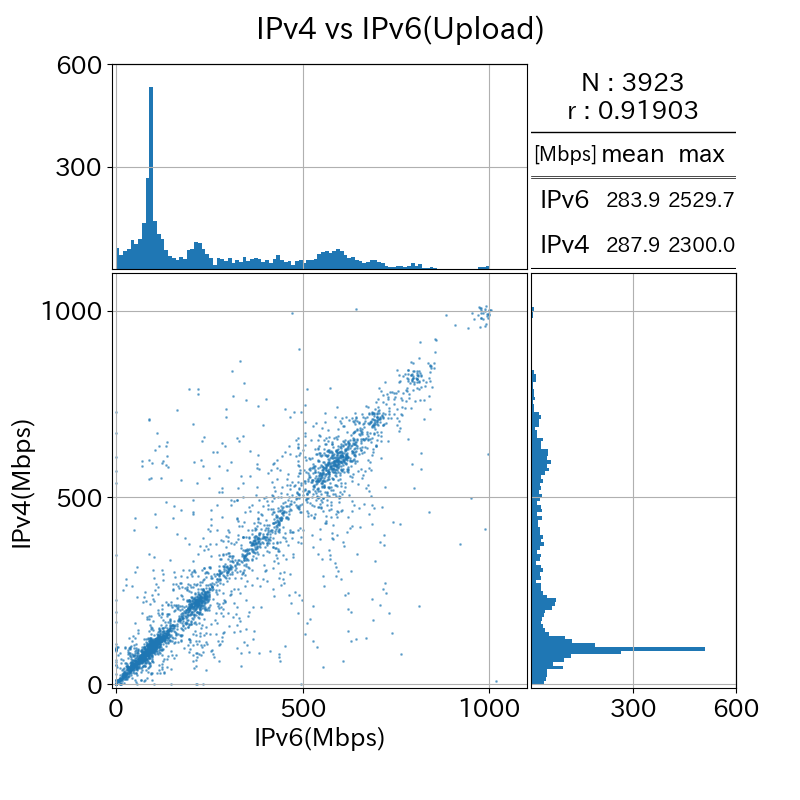
\includegraphics[width=0.85\textwidth]{fig/new_KDDI_ul.png}
                    \subcaption{B社の場合}
                    \label{new_KDDI_ul}
                \end{subfigure}
                \begin{subfigure}[b]{\textwidth}
                    \centering
                    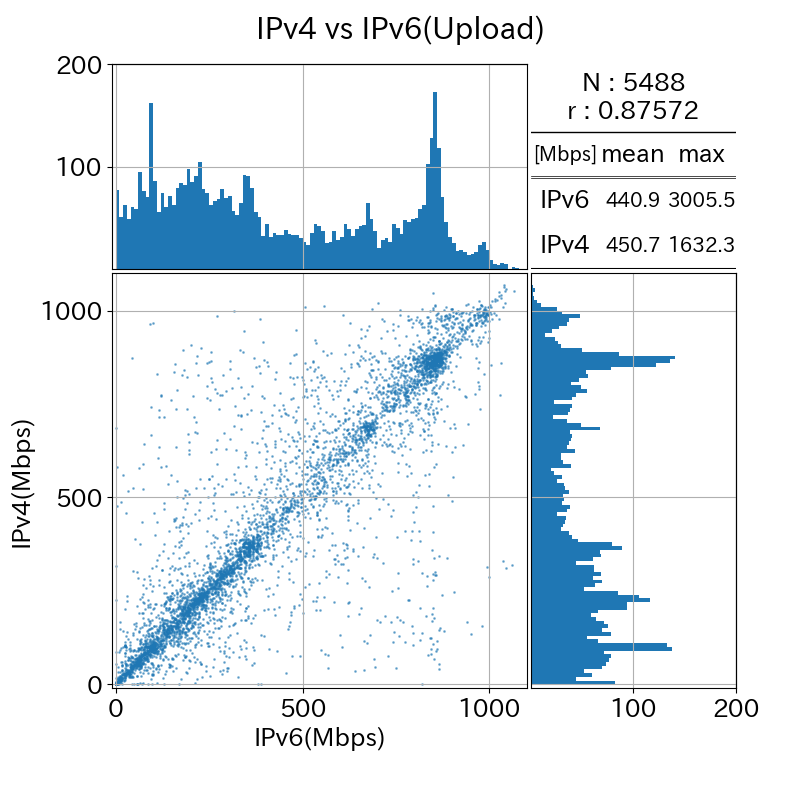
\includegraphics[width=0.85\textwidth]{fig/new_Sony_ul.png}
                    \subcaption{C社の場合}
                    \label{new_Sony_ul}
                \end{subfigure}
                \caption{ISPの違いによる\\アップロードのスループット}
                \label{fig:new_isp_ul2}
            \end{center}
        \end{minipage}
    \end{center}
\end{figure}
\FloatBarrier
%\end{comment}

%%%%%%%%%%%%%%%%%%%%%%%%%%%%%%%%%%%%%%%%%%%%%%%%%%%%%%%%%%%%%%%%%%%%%%%%%%
\subsection{アクセス網の種類によるスループットへの影響}
次にアクセス網の種類によるスループットへの影響について述べる.\cref{fig:old_Line_dl,fig:new_Line_dl}はダウンロードのスループットのグラフ,\cref{fig:old_Line_ul,fig:new_Line_ul}はアップロードのスループットのグラフである.\cref{old_FTTH_dl,new_FTTH_dl}はそれぞれの期間でFTTHを使用した場合のダウンロードのスループットである.両者とも100Mbps付近にピークが表れて緩やかにデータ数が減っていくふるまいを見せている.これはアップロードの場合も類似する振る舞いをしている.一方,\cref{old_CATV_dl,new_CATV_dl}のCATVを使用した場合はピークが表れる位置がFTTHと異なり,ダウンロードの場合は340Mbps付近に表れる.アップロードの場合は10Mbpsにピークが表れている.CATVを使用したインターネット接続サービスについて調査すると,ダウンロードのスループットが最大340Mbps,アップロードのスループットが最大10Mbpsであると述べているサービスがいくつか確認された.このことからアクセス網の種類によってスループットの限界が異なることがわかる.さらに\cref{new_Mobile_dl,new_Mobile_ul}のMobileの場合は10Mbps付近にピークが表れている.Mobileを使用した場合のスループットの限界はFTTHやCATVに比べて低いことがわかる.ただし,\cref{old_CATV_dl,new_CATV_dl}を比較すると,340Mbpsのピークの前後のヒストグラムの振る舞いが異なる.ピークの前後のデータの割合は\cref{tab:catv}のように変化し340Mbps以上のデータが約20\%増加している.CATVによる配信サービスについて調べると,旧来使用されてきたHFC(Hybrid Fiber-Coaxial)方式や同軸方式を光ファイバーに置き換える動き\cite{nagaoka}が進んでおり,総務省の資料\cite{catv}によると約80\%の事業者がFTTH方式を採用していることがわかった.このことから,アクセス網の種類だけでなくアクセス環境全体が時期によって変化していることがわかる.
以上のことからアクセス網の種類によってスループットの限界が異なることがわかったが,その振る舞いは時期によって異なることがわかる.

%\begin{comment}
\begin{figure}[htbp]
    %\centering
    \begin{center}
        % 左側の図
        \begin{minipage}[t]{0.48\textwidth}
            \begin{center}
                \begin{subfigure}[b]{\textwidth}
                    \centering
                    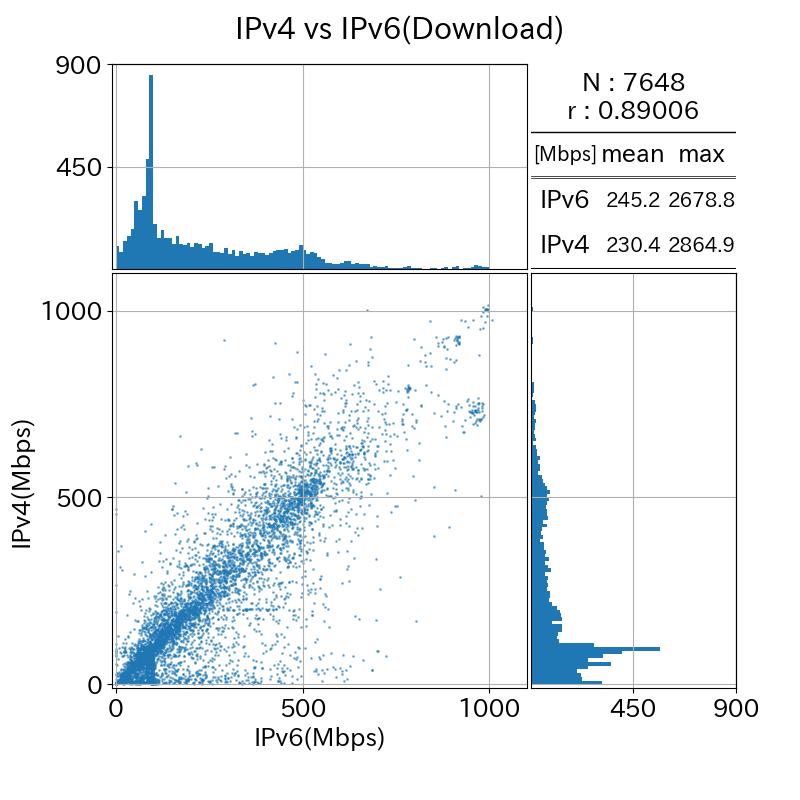
\includegraphics[width=0.85\textwidth]{fig/old_FTTH_dl.png}
                    \subcaption{FTTHを使用した場合}
                    \label{old_FTTH_dl}
                \end{subfigure}
                \begin{subfigure}[b]{\textwidth}
                    \centering
                    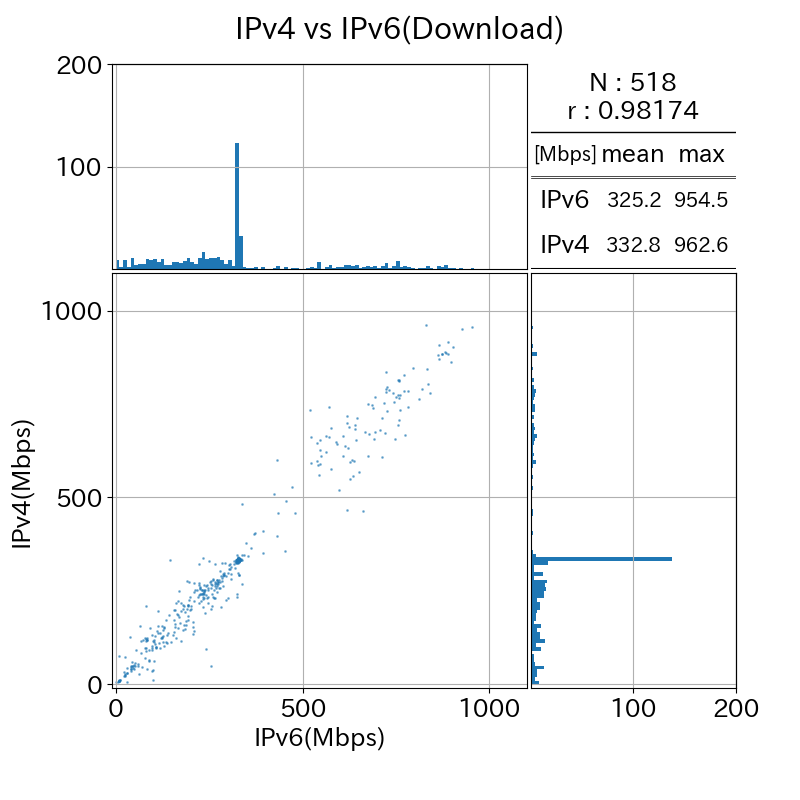
\includegraphics[width=0.85\textwidth]{fig/old_CATV_dl.png}
                    \subcaption{CATVを使用した場合}
                    \label{old_CATV_dl}
                \end{subfigure}
                \begin{subfigure}[b]{\textwidth}
                    \centering
                    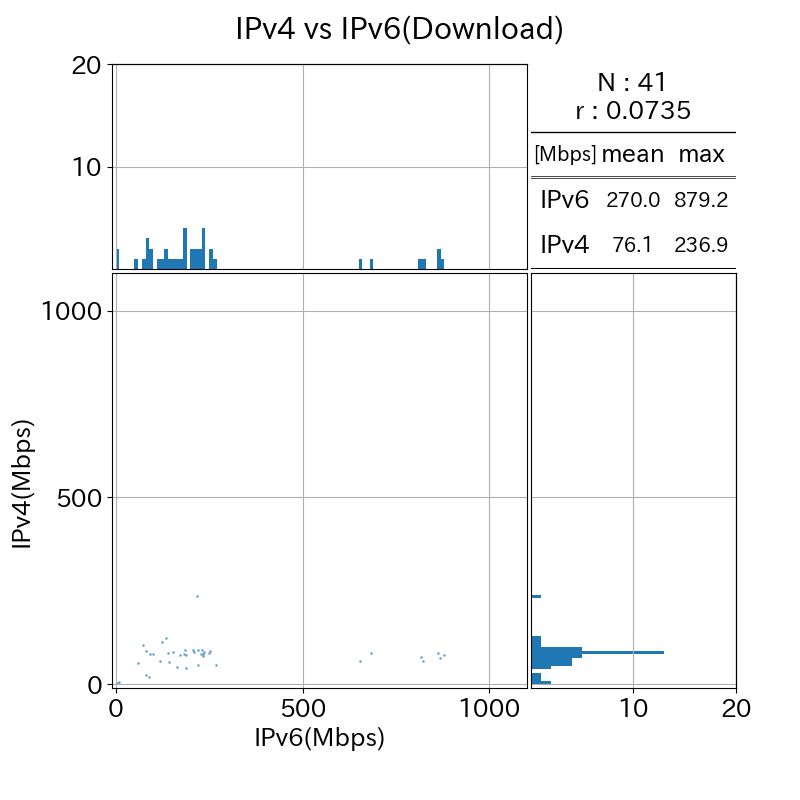
\includegraphics[width=0.85\textwidth]{fig/old_Mobile_dl.png}
                    \subcaption{Mobileを使用した場合}
                    \label{old_Mobile_dl}
                \end{subfigure}
            \caption{(1)のダウンロードのスループット}
            \label{fig:old_Line_dl}
            \end{center}
        \end{minipage}
        \hfill
        \begin{minipage}[t]{0.48\textwidth}
            \begin{subfigure}[b]{\textwidth}
                \centering
                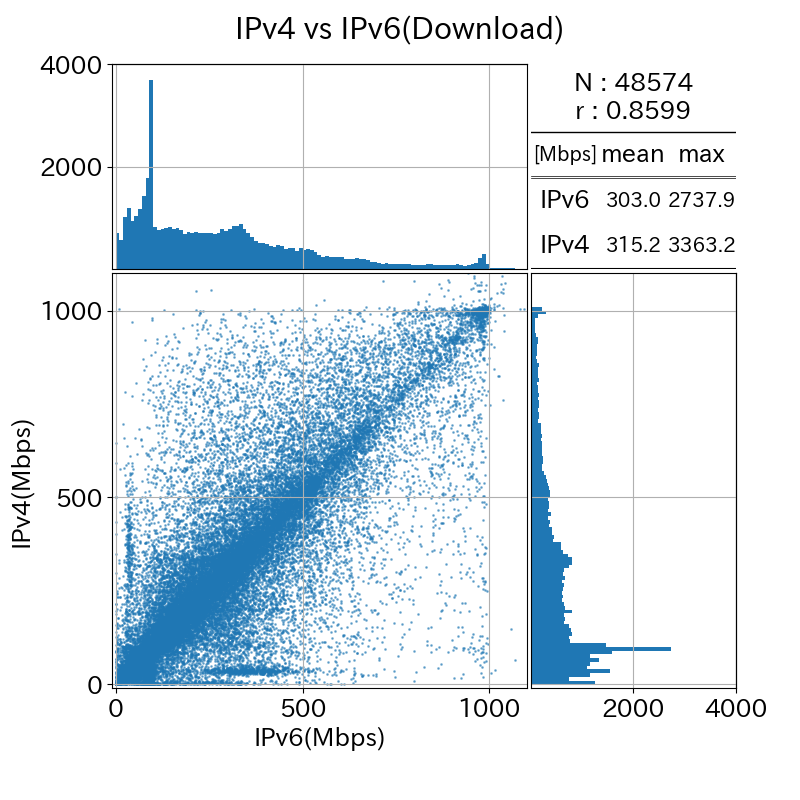
\includegraphics[width=0.85\textwidth]{fig/new_FTTH_dl.png}
                \subcaption{FTTHを使用した場合}
                \label{new_FTTH_dl}
            \end{subfigure}
            \begin{subfigure}[b]{\textwidth}
                \centering
                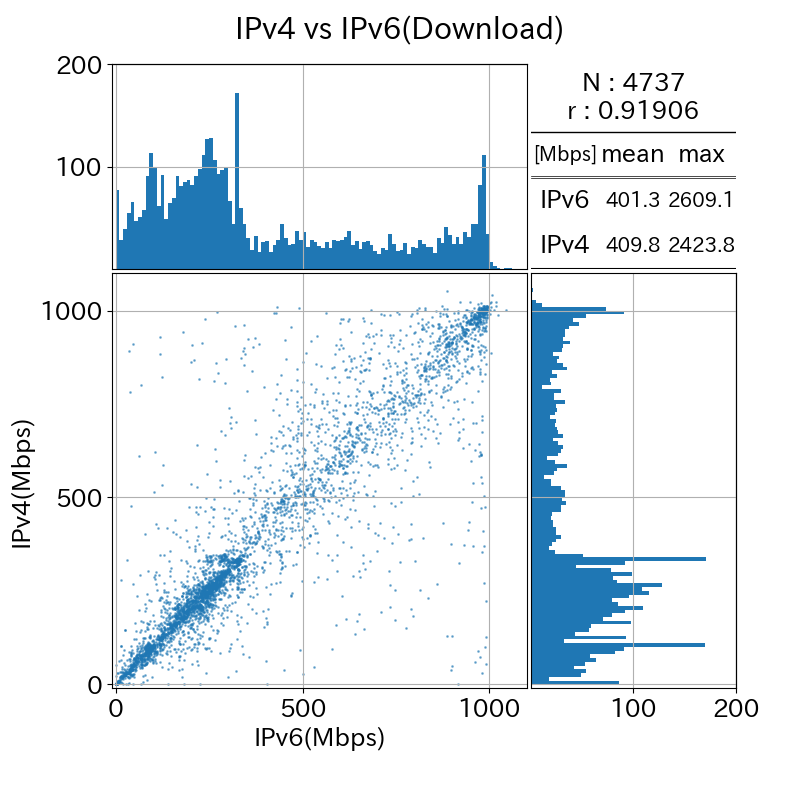
\includegraphics[width=0.85\textwidth]{fig/new_CATV_dl.png}
                \subcaption{CATVを使用した場合}
                \label{new_CATV_dl}
            \end{subfigure}
            \begin{subfigure}[b]{\textwidth}
                \centering
                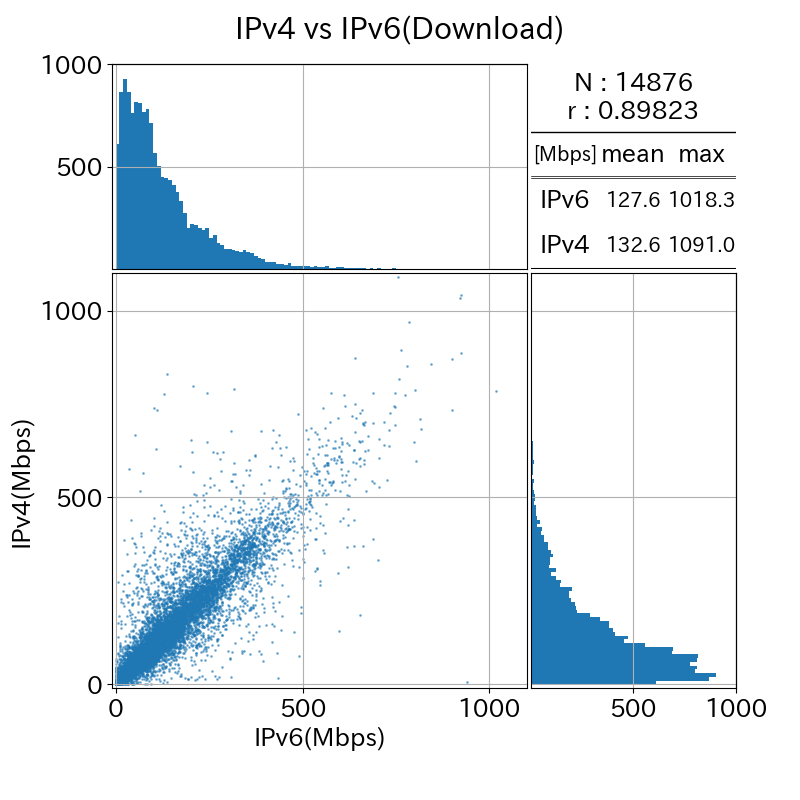
\includegraphics[width=0.85\textwidth]{fig/new_Mobile_dl.png}
                \subcaption{Mobileを使用した場合}
                \label{new_Mobile_dl}
            \end{subfigure}
            \caption{(2)のダウンロードのスループット}
            \label{fig:new_Line_dl}
        \end{minipage}
    \end{center}
\end{figure}
\FloatBarrier

\begin{figure}[htbp]
    %\centering
    \begin{center}
        % 左側の図
        \begin{minipage}[t]{0.48\textwidth}
            \begin{center}
                \begin{subfigure}[b]{\textwidth}
                    \centering
                    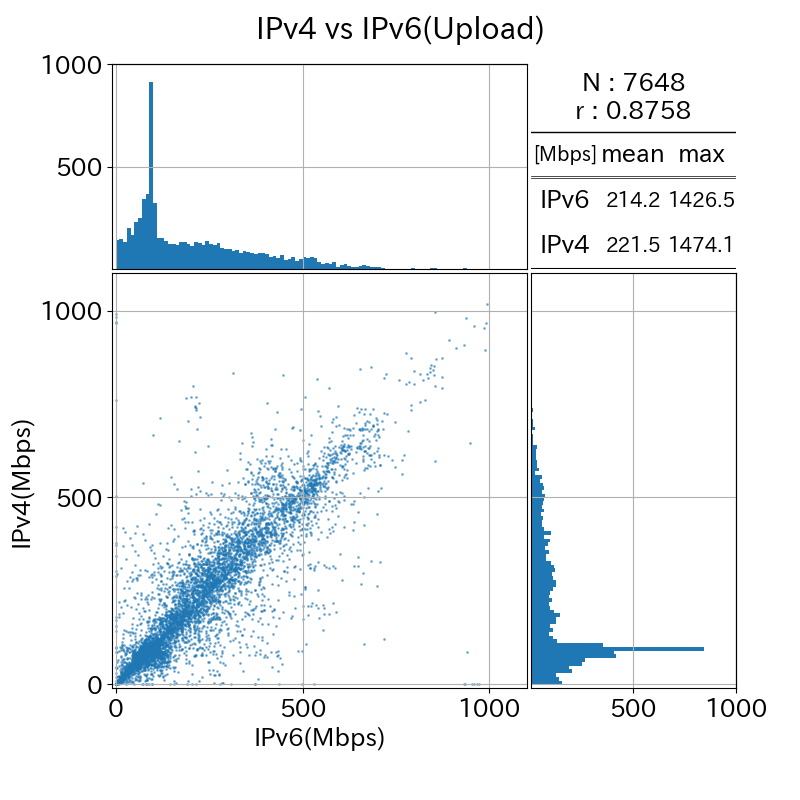
\includegraphics[width=0.85\textwidth]{fig/old_FTTH_ul.png}
                    \subcaption{FTTHを使用した場合}
                    \label{old_FTTH_ul}
                \end{subfigure}
                \begin{subfigure}[b]{\textwidth}
                    \centering
                    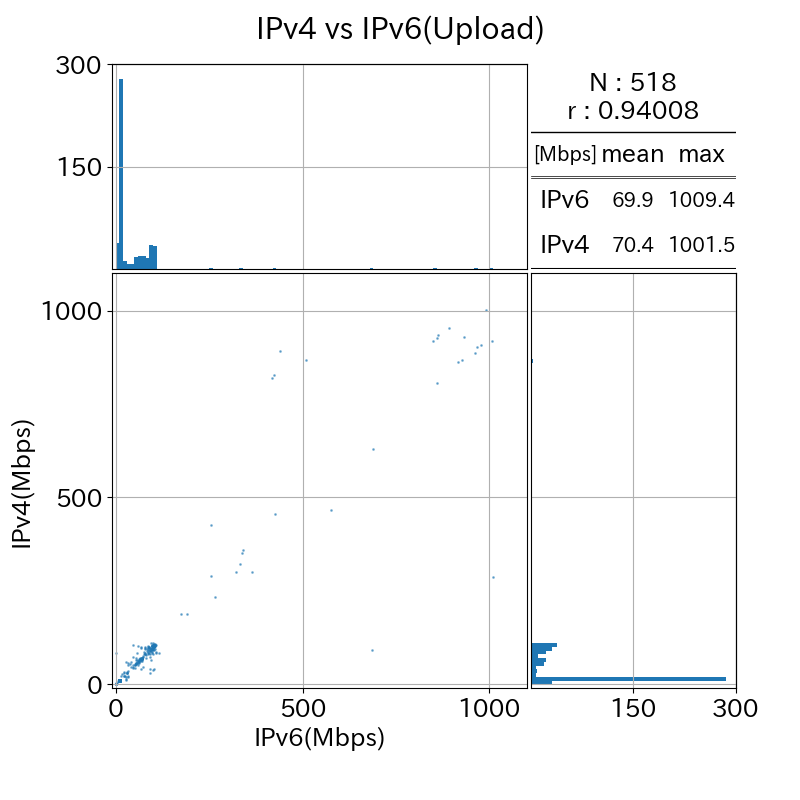
\includegraphics[width=0.85\textwidth]{fig/old_CATV_ul.png}
                    \subcaption{CATVを使用した場合}
                    \label{old_CATV_ul}
                \end{subfigure}
                \begin{subfigure}[b]{\textwidth}
                    \centering
                    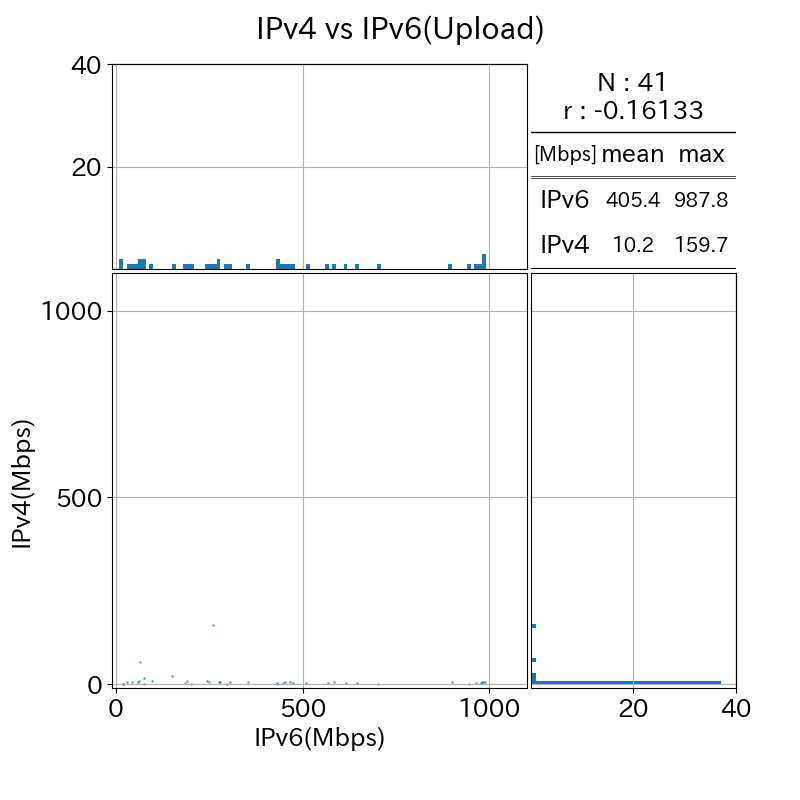
\includegraphics[width=0.85\textwidth]{fig/old_Mobile_ul.png}
                    \subcaption{Mobileを使用した場合}
                    \label{old_Mobile_ul}
                \end{subfigure}
            \caption{(1)のアップロードのスループット}
            \label{fig:old_Line_ul}
            \end{center}
        \end{minipage}
        \hfill
        \begin{minipage}[t]{0.48\textwidth}
            \begin{subfigure}[b]{\textwidth}
                \centering
                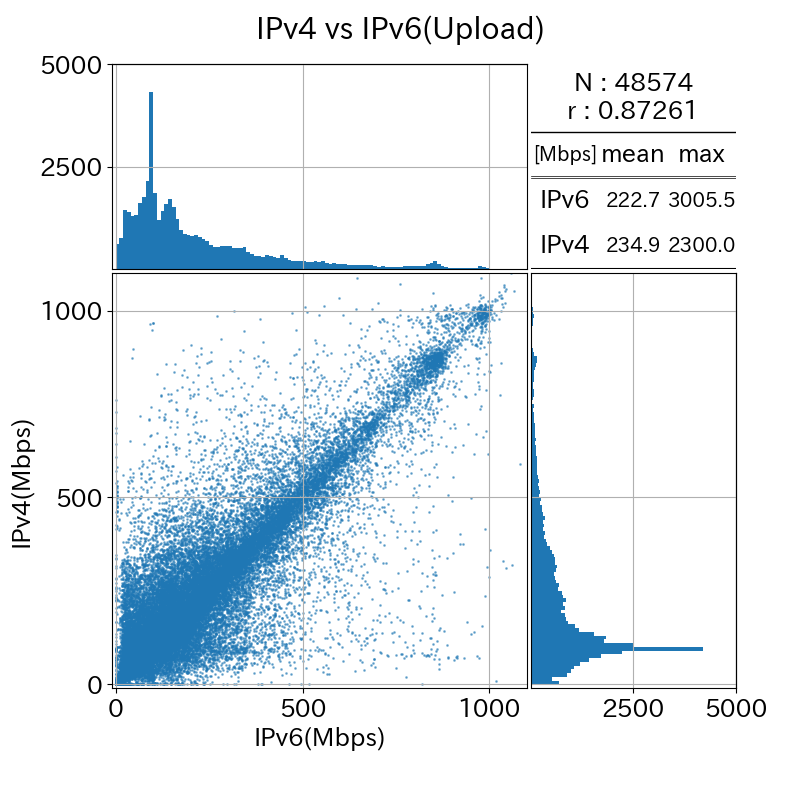
\includegraphics[width=0.85\textwidth]{fig/new_FTTH_ul.png}
                \subcaption{FTTHを使用した場合}
                \label{new_FTTH_ul}
            \end{subfigure}
            \begin{subfigure}[b]{\textwidth}
                \centering
                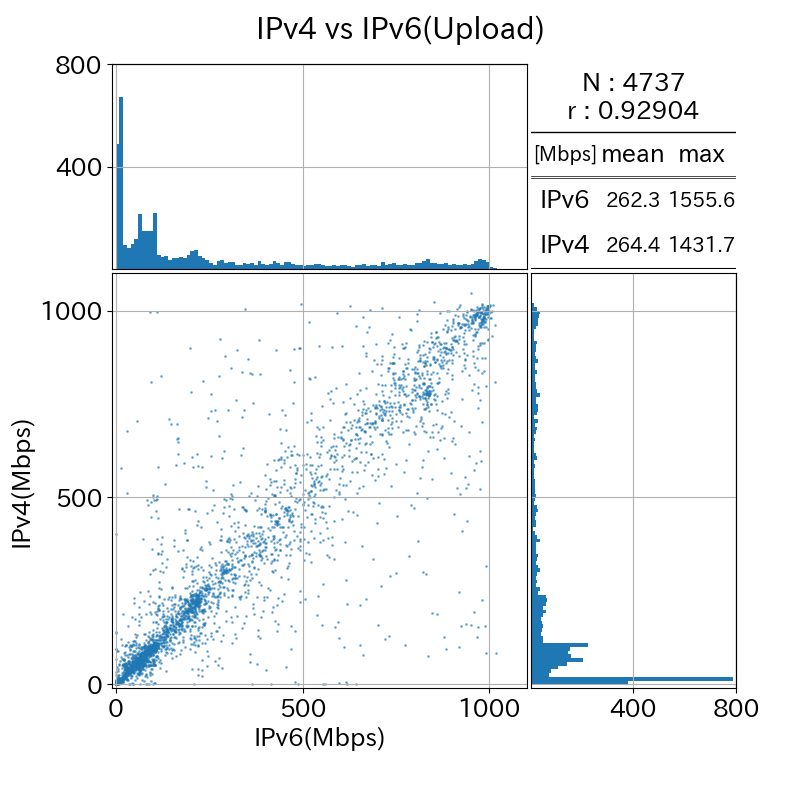
\includegraphics[width=0.85\textwidth]{fig/new_CATV_ul.png}
                \subcaption{CATVを使用した場合}
                \label{new_CATV_ul}
            \end{subfigure}
            \begin{subfigure}[b]{\textwidth}
                \centering
                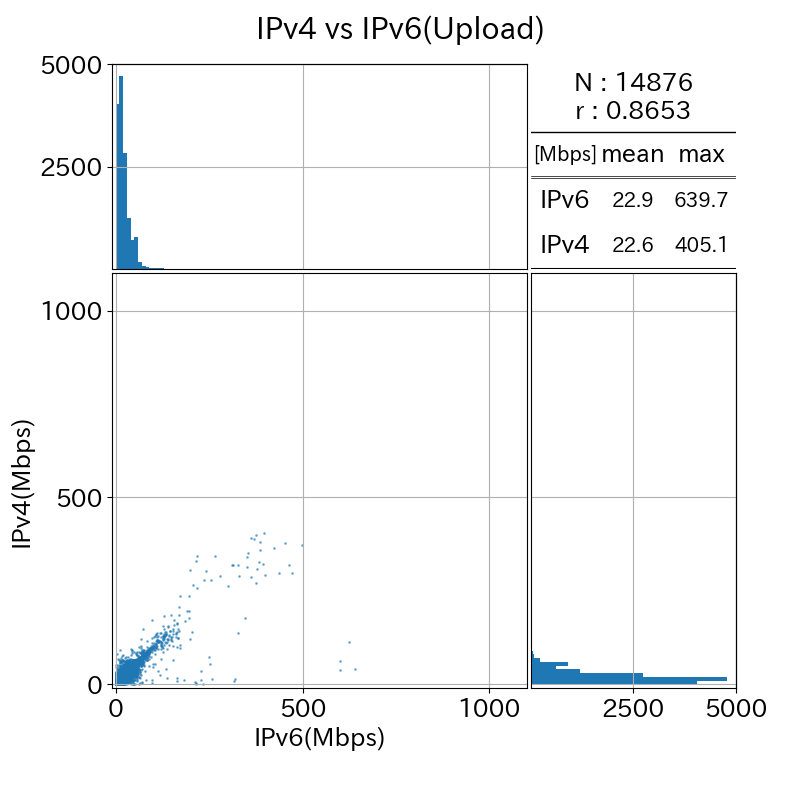
\includegraphics[width=0.85\textwidth]{fig/new_Mobile_ul.png}
                \subcaption{Mobileを使用した場合}
                \label{new_Mobile_ul}
            \end{subfigure}
            \caption{(2)のアップロードのスループット}
            \label{fig:new_Line_ul}
        \end{minipage}
    \end{center}
\end{figure}
\FloatBarrier

\begin{table}[htbp]
    \caption{CATVのピーク前後のデータの割合}
    \label{tab:catv}
    \begin{center}
        \begin{tabular}{ccc} \hline
            期間 & 340Mbps未満のデータの割合 & 340Mbps以上のデータの割合 \\ \hline \hline
            (1) & 77.11\% & 22.89\% \\
            (2) & 57.84\% & 42.16\% \\ \hline
        \end{tabular}
    \end{center}
\end{table}
\FloatBarrier
%\end{comment}

%%%%%%%%%%%%%%%%%%%%%%%%%%%%%%%%%%%%%%%%%%%%%%%%%%%%%%%%%%%%%%%%%%%%%%%%%%
\subsection{インターネット接続方式によるスループットへの影響}
最後にインターネット接続方式によるスループットへの影響について述べる.\cref{fig:old_connect_dl,fig:new_connect_dl}はそれぞれの期間のダウンロードのスループットのグラフ,\cref{fig:old_connect_ul,fig:new_connect_ul}はアップロードのスループットのグラフである.\subref{old_IPv4aaS_dl}から\subref{old_PPPoE_dl}の平均値を比較するとIPv4とIPv6の両者とも異なる値を示している.ここで\subref{old_IPv4aaS_dl}と\subref{old_mix_dl}の条件の違いはIPv4の接続方式であるにも関わらず,IPv6のスループットの平均値も異なる.同様に\subref{old_mix_dl}と\subref{old_PPPoE_dl}の条件の違いはIPv6の接続方式であるにも関わらず,IPv4のスループットの平均値も異なる.このことからインターネットの接続方式による振る舞いの違いが表れるだけでなく,IPv4/IPv6の接続方式の組み合わせによっても振る舞いが異なることがわかる.しかし,この影響の要因は他にも検証が必要であると考える.

%\begin{comment}
\begin{figure}[htbp]
    %\centering
    \begin{center}
        % 左側の図
        \begin{minipage}[t]{0.48\textwidth}
            \begin{subfigure}[b]{\textwidth}
                \centering
                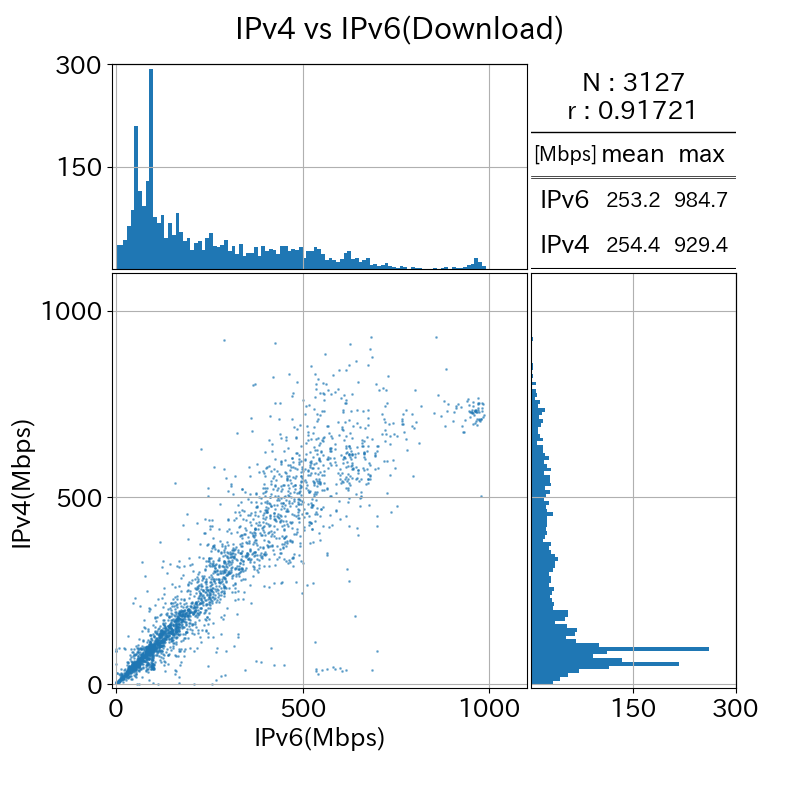
\includegraphics[width=0.8\textwidth]{fig/old_IPv4aaS_dl.png}
                \subcaption{IPv4/IPv6でIPoEを使用した場合}
                \label{old_IPv4aaS_dl}
            \end{subfigure}
            \begin{subfigure}[b]{\textwidth}
                \centering
                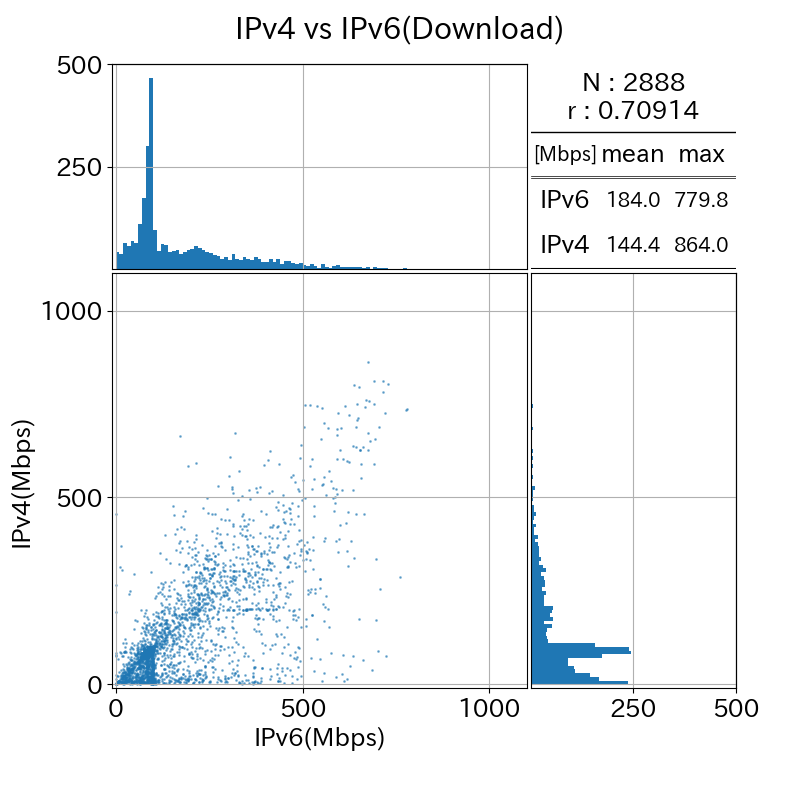
\includegraphics[width=0.8\textwidth]{fig/old_mix_dl.png}
                \subcaption{IPv4はPPPoE,IPv6はIPoEを\\使用した場合}
                \label{old_mix_dl}
            \end{subfigure}
            \begin{subfigure}[b]{\textwidth}
                \centering
                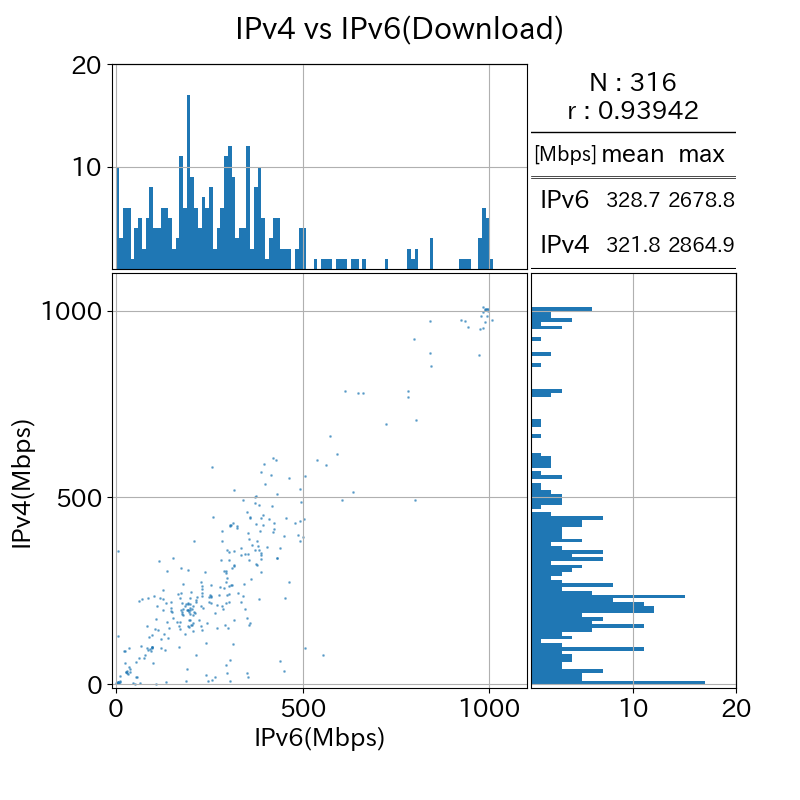
\includegraphics[width=0.8\textwidth]{fig/old_PPPoE_dl.png}
                \subcaption{IPv4/IPv6でPPPoEを使用した場合}
                \label{old_PPPoE_dl}
            \end{subfigure}
        \caption{(1)のダウンロードのスループット}
        \label{fig:old_connect_dl}
        \end{minipage}
        \hfill
        \begin{minipage}[t]{0.48\textwidth}
            \begin{subfigure}[b]{\textwidth}
                \centering
                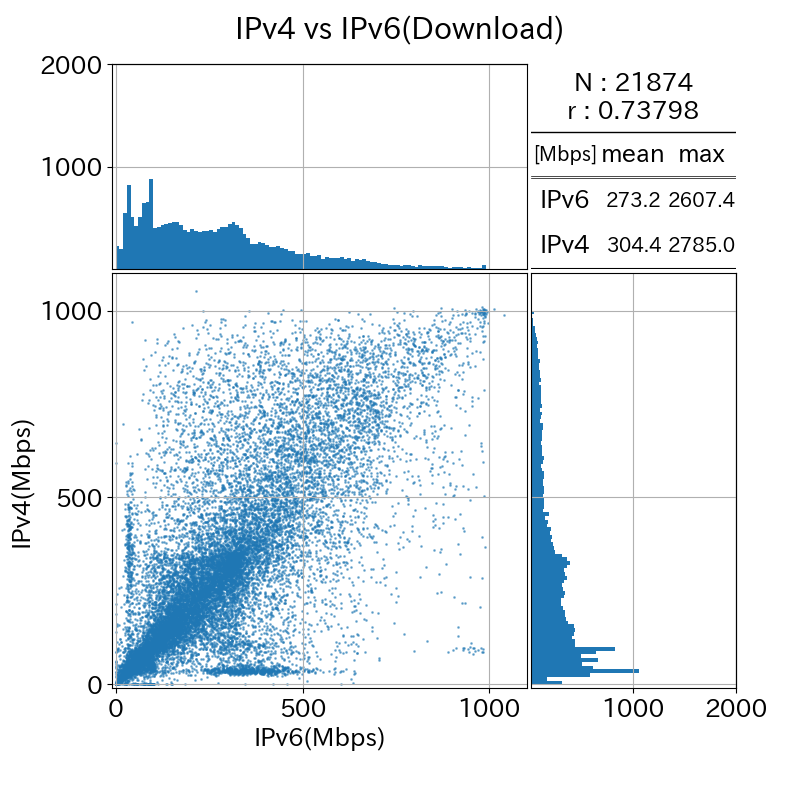
\includegraphics[width=0.8\textwidth]{fig/new_IPv4aaS_dl.png}
                \subcaption{IPv4/IPv6でIPoEを使用した場合}
                \label{new_IPv4aaS_dl}
            \end{subfigure}
            \begin{subfigure}[b]{\textwidth}
                \centering
                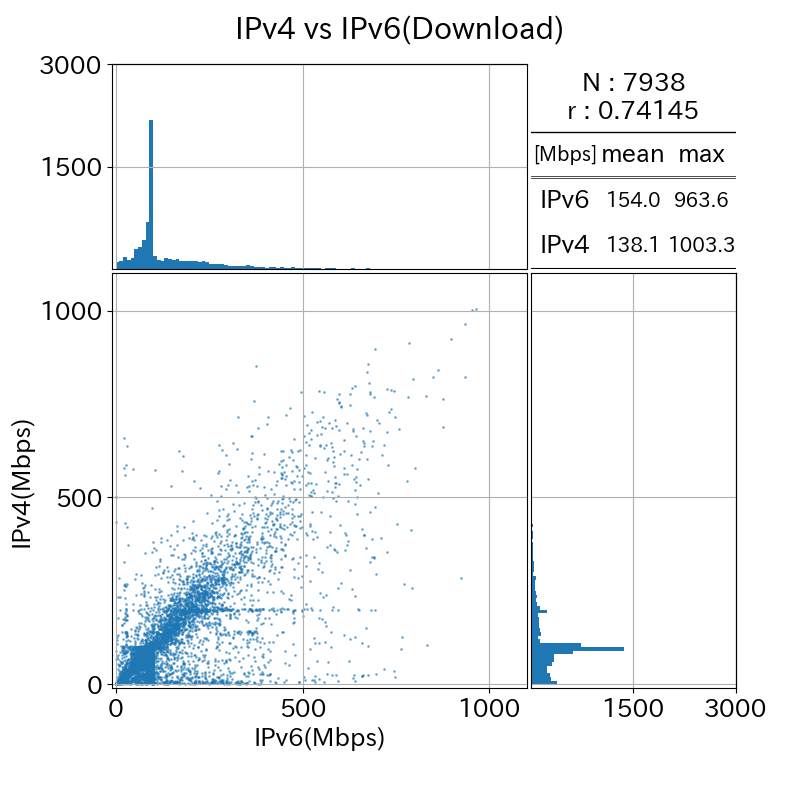
\includegraphics[width=0.8\textwidth]{fig/new_mix_dl.png}
                \subcaption{IPv4はPPPoE,IPv6はIPoEを使用した場合}
                \label{new_mix_dl}
            \end{subfigure}
            \begin{subfigure}[b]{\textwidth}
                \centering
                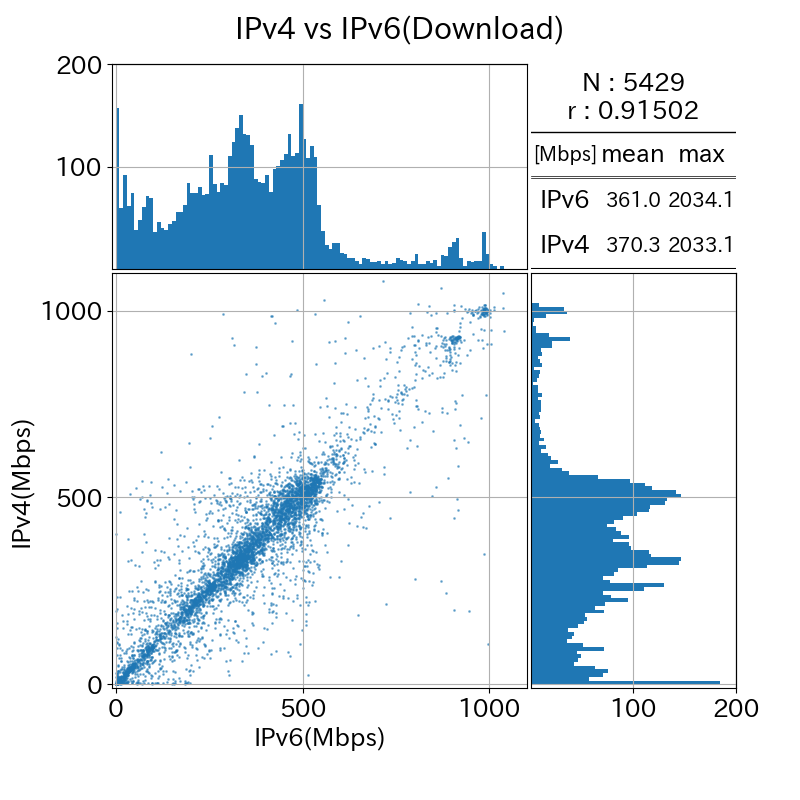
\includegraphics[width=0.8\textwidth]{fig/new_PPPoE_dl.png}
                \subcaption{IPv4/IPv6でPPPoEを使用した場合}
                \label{new_PPPoE_dl}
            \end{subfigure}
            \caption{(2)のダウンロードのスループット}
            \label{fig:new_connect_dl}
        \end{minipage}
    \end{center}
\end{figure}
\FloatBarrier

\begin{figure}[htbp]
    %\centering
    \begin{center}
        % 左側の図
        \begin{minipage}[t]{0.48\textwidth}
            \begin{center}
                \begin{subfigure}[b]{\textwidth}
                    \centering
                    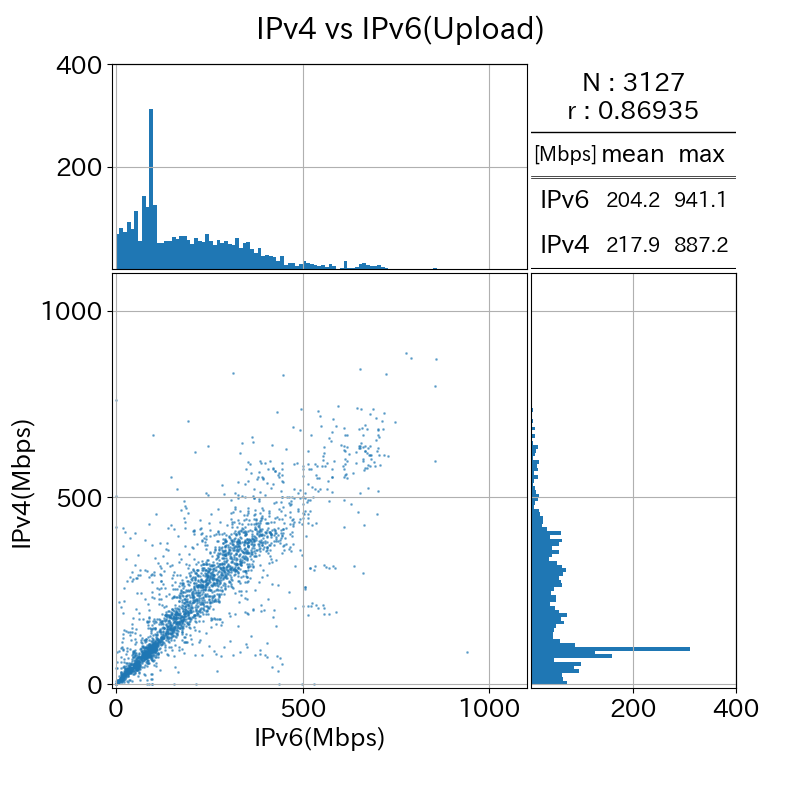
\includegraphics[width=0.8\textwidth]{fig/old_IPv4aaS_ul.png}
                    \subcaption{IPv4/IPv6でIPoEを使用した場合}
                    \label{old_IPv4aaS_ul}
                \end{subfigure}
                \begin{subfigure}[b]{\textwidth}
                    \centering
                    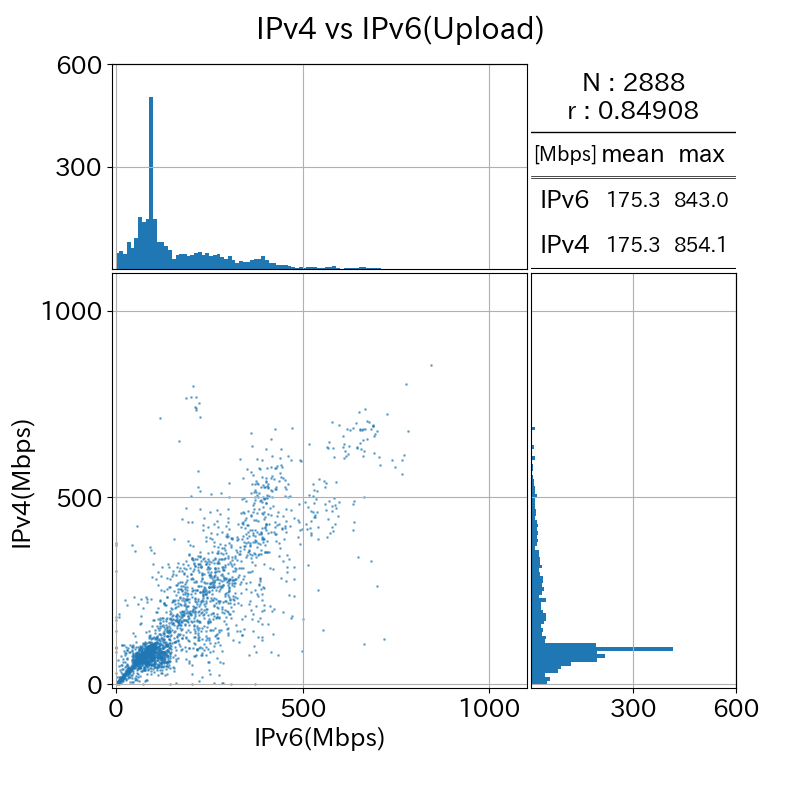
\includegraphics[width=0.8\textwidth]{fig/old_mix_ul.png}
                    \subcaption{IPv4はPPPoE,IPv6はIPoEを使用した場合}
                    \label{old_mix_ul}
                \end{subfigure}
                \begin{subfigure}[b]{\textwidth}
                    \centering
                    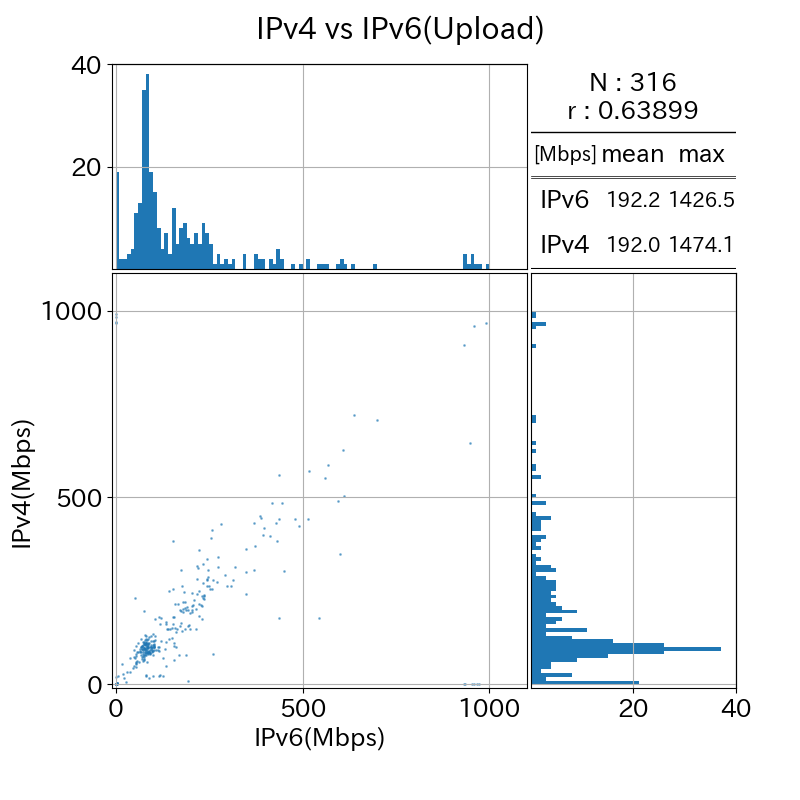
\includegraphics[width=0.8\textwidth]{fig/old_PPPoE_ul.png}
                    \subcaption{IPv4/IPv6でPPPoEを使用した場合}
                    \label{old_PPPoE_ul}
                \end{subfigure}
            \caption{(1)のアップロードのスループット}
            \label{fig:old_connect_ul}
            \end{center}
        \end{minipage}
        \hfill
        \begin{minipage}[t]{0.48\textwidth}
            \begin{subfigure}[b]{\textwidth}
                \centering
                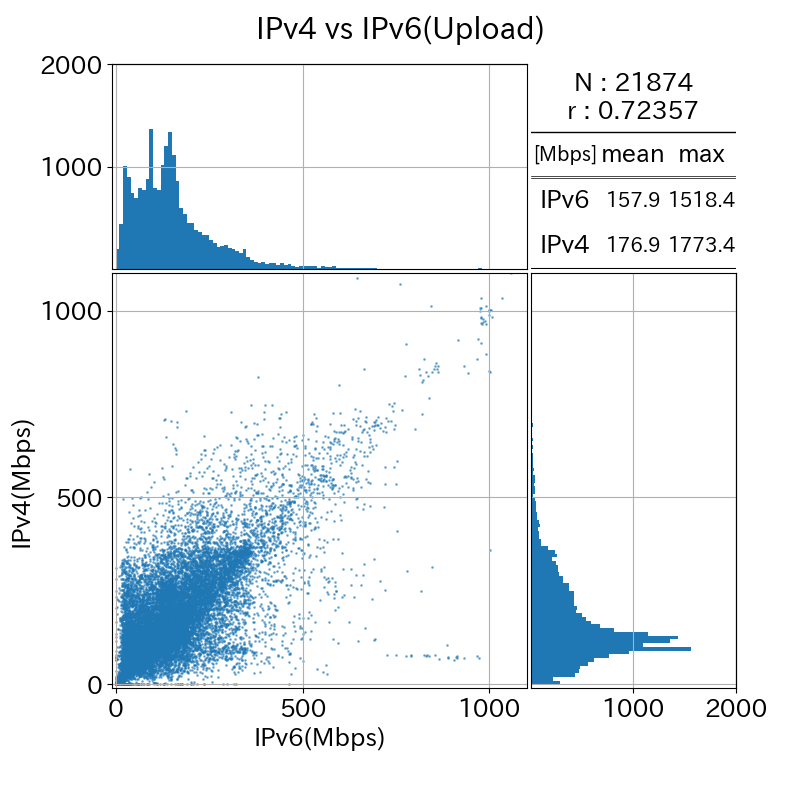
\includegraphics[width=0.8\textwidth]{fig/new_IPv4aaS_ul.png}
                \subcaption{IPv4/IPv6でIPoEを使用した場合}
                \label{new_IPv4aaS_ul}
            \end{subfigure}
            \begin{subfigure}[b]{\textwidth}
                \centering
                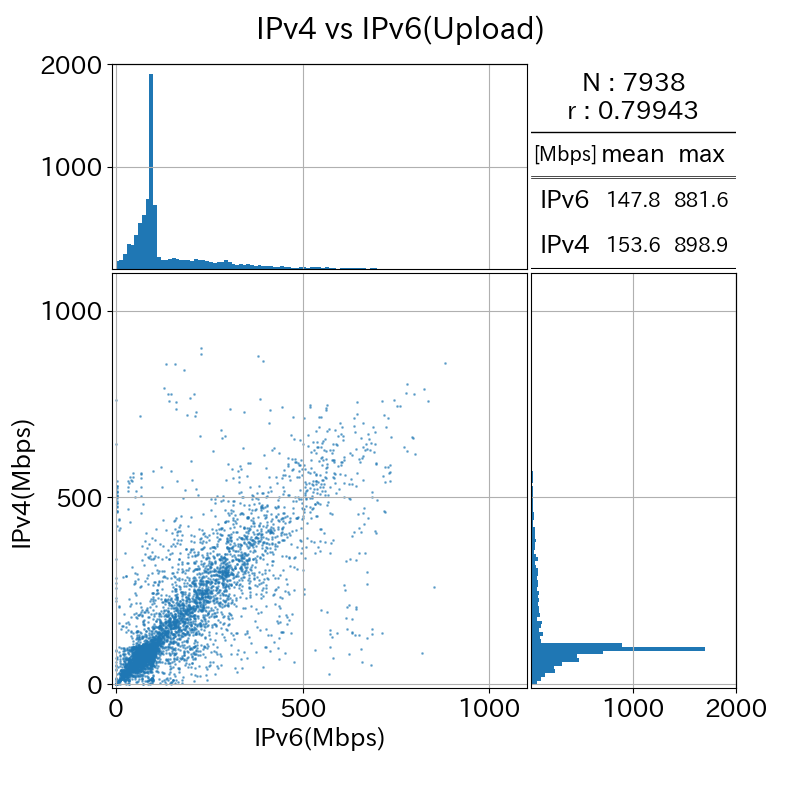
\includegraphics[width=0.8\textwidth]{fig/new_mix_ul.png}
                \subcaption{IPv4はPPPoE,IPv6はIPoEを使用した場合}
                \label{new_mix_ul}
            \end{subfigure}
            \begin{subfigure}[b]{\textwidth}
                \centering
                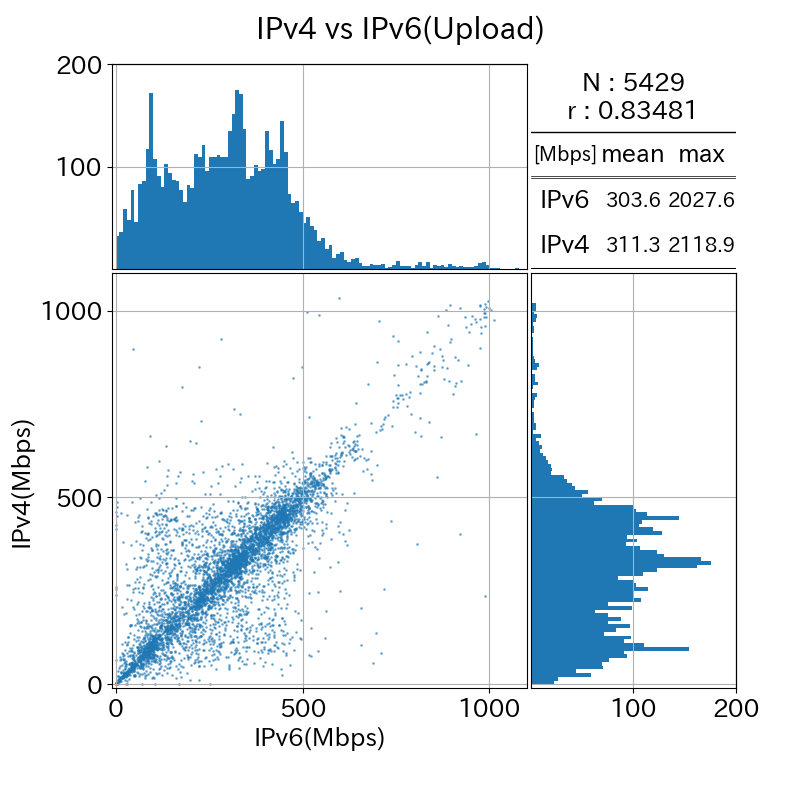
\includegraphics[width=0.8\textwidth]{fig/new_PPPoE_ul.png}
                \subcaption{IPv4/IPv6でPPPoEを使用した場合}
                \label{new_PPPoE_ul}
            \end{subfigure}
            \caption{(2)のアップロードのスループット}
            \label{fig:new_connect_ul}
        \end{minipage}
    \end{center}
\end{figure}
\FloatBarrier
%\end{comment}

%%%%%%%%%%%%%%%%%%%%%%%%%%%%%%%%%%%%%%%%%%%%%%%%%%%%%%%%%%%%%%%%%%%%%%%%%%
\section{RTTの調査}
\label{sec:rtt}
\cref{sec:throughput}と同様の手法を用いてRTTについて調査した.
\subsection{ISPの網によるRTTへの影響}
\cref{fig:old_isp_rtt,fig:new_isp_rtt}はそれぞれの期間のISPの網の違いによるRTTの比較を示す.\cref{old_sameISP_rtt,new_sameISP_rtt}は同じISPを使用した場合の結果で,\cref{old_diffISP_rtt,new_diffISP_rtt}は異なるISPを使用した場合の結果である.これらの間に振る舞いの違いは見られないことがわかった.

%%%%%%%%%%%%%%%%%%%%%%%%%%%%%%%%%%%%%%%%%%%%%%%%%%%%%%%%%%%%%%%%%%%%%%%%%%

\subsection{アクセス網の種類によるRTTへの影響}
\cref{fig:old_Line_rtt,fig:new_Line_rtt}はそれぞれの期間のアクセス網の種類によるRTTの比較を示す.\cref{old_FTTH_rtt,new_FTTH_rtt}がFTTHを使用した場合,\cref{old_CATV_rtt,new_CATV_rtt}はCATVを使用した場合,\cref{old_Mobile_rtt,new_Mobile_rtt}はMobileを使用した場合の結果である.FTTHとCATVを使用した場合のRTTはほぼ同じ振る舞いをしていると言える.一方,Mobileを使用した場合のRTTはFTTHやCATVに比べてRTTの平均値が大きい.平均値だけでなく,散布図の分布やヒストグラムのピークの場所からわかる.

%%%%%%%%%%%%%%%%%%%%%%%%%%%%%%%%%%%%%%%%%%%%%%%%%%%%%%%%%%%%%%%%%%%%%%%%%%
\subsection{インターネット接続方式によるRTTへの影響}
\cref{fig:old_connect_rtt,fig:new_connect_rtt}はそれぞれの期間のインターネット接続方式によるRTTの比較を示す.\cref{old_IPv4aaS_rtt,new_IPv4aaS_rtt}はIPv4/IPv6でIPoEを使用した場合,\cref{old_mix_rtt,new_mix_rtt}はIPv4はPPPoE,IPv6はIPoEを使用した場合,\cref{old_PPPoE_rtt,new_PPPoE_rtt}はIPv4/IPv6でPPPoEを使用した場合の結果である.これらの間も振る舞いの違いは見られないことがわかった.

%\begin{comment}
\begin{figure}[htbp]
    \begin{center}
        \begin{subfigure}[b]{0.49\textwidth}
            \centering
            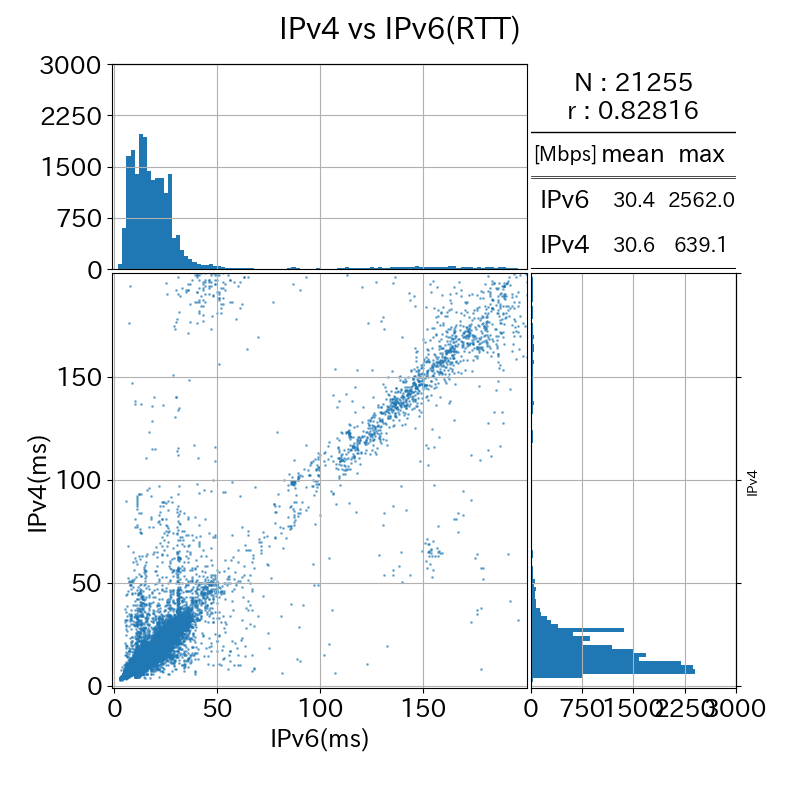
\includegraphics[width=1.0\textwidth]{fig/old_sameISP_rtt.png}
            \subcaption{同じISPを使用した場合}
            \label{old_sameISP_rtt}
        \end{subfigure}
        \begin{subfigure}[b]{0.49\textwidth}
            \centering
            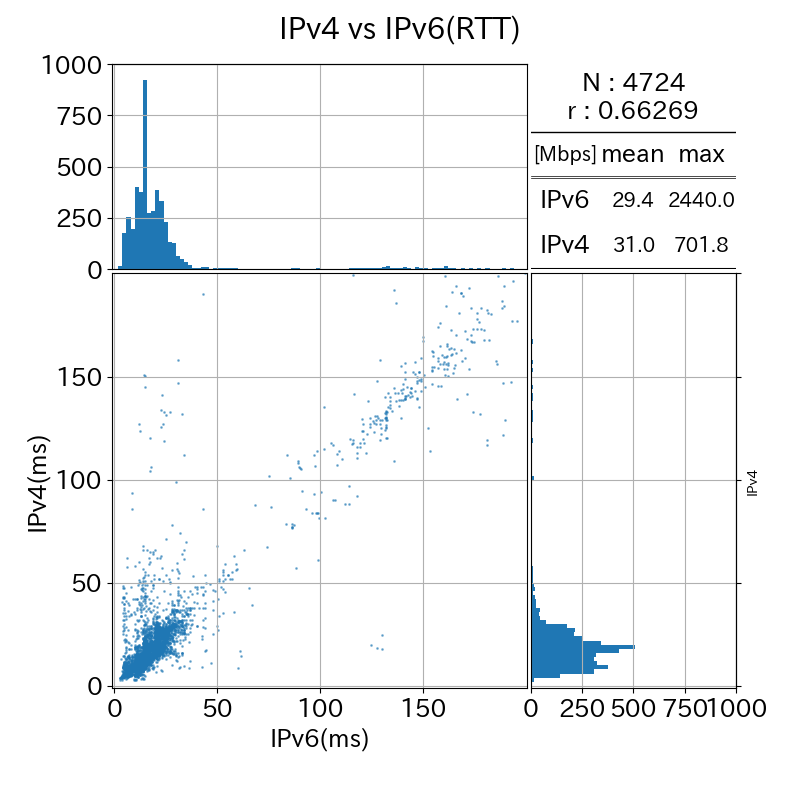
\includegraphics[width=1.0\textwidth]{fig/old_diffISP_rtt.png}
            \subcaption{異なるISPを使用した場合}
            \label{old_diffISP_rtt}
        \end{subfigure}
        \caption{(1)のRTT}
        \label{fig:old_isp_rtt}
    
        \begin{subfigure}[b]{0.49\textwidth}
            \centering
            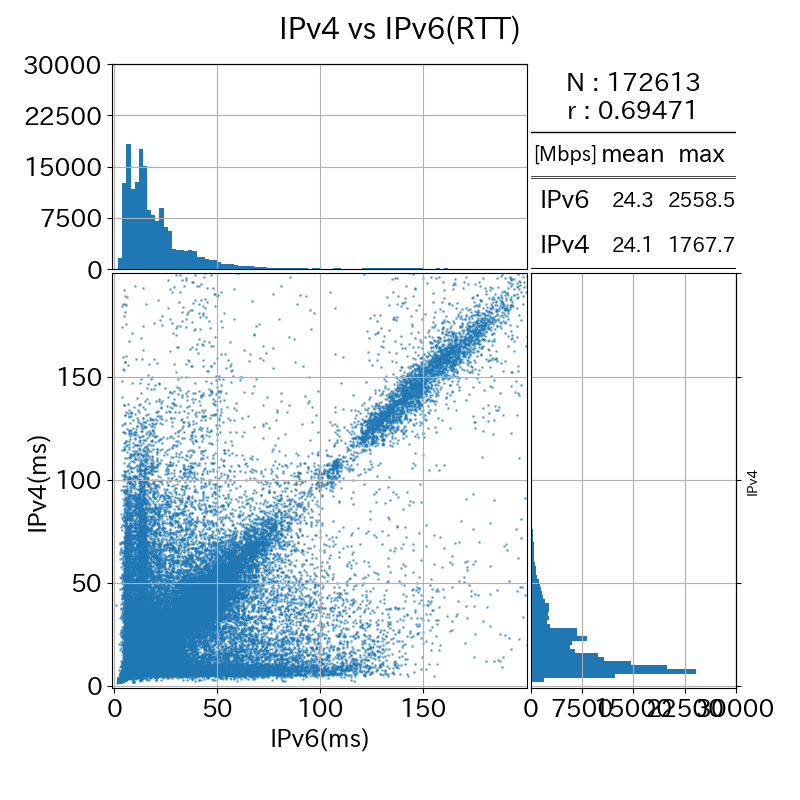
\includegraphics[width=1.0\textwidth]{fig/new_sameISP_rtt.png}
            \subcaption{同じISPを使用した場合}
            \label{new_sameISP_rtt}
        \end{subfigure}
        \begin{subfigure}[b]{0.49\textwidth}
            \centering
            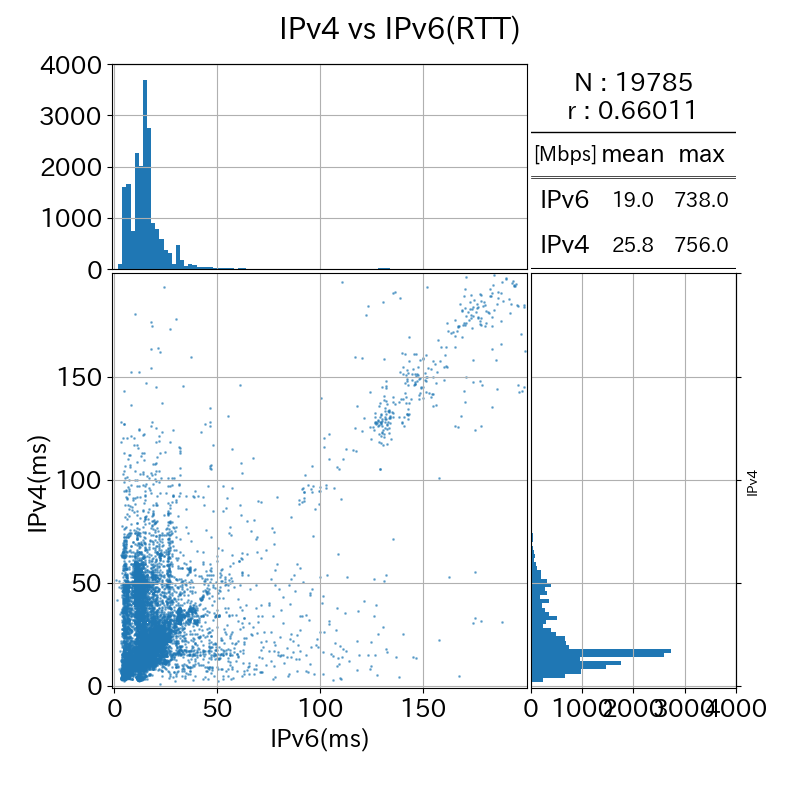
\includegraphics[width=1.0\textwidth]{fig/new_diffISP_rtt.png}
            \subcaption{異なるISPを使用した場合}
            \label{new_diffISP_rtt}
        \end{subfigure}
        \caption{(2)のRTT}
        \label{fig:new_isp_rtt}
    \end{center}
\end{figure}
\FloatBarrier
%\end{comment}

%\begin{comment}
\begin{figure}[htbp]
    %\centering
    \begin{center}
        % 左側の図
        \begin{minipage}[t]{0.48\textwidth}
            \begin{center}
                \begin{subfigure}[b]{\textwidth}
                    \centering
                    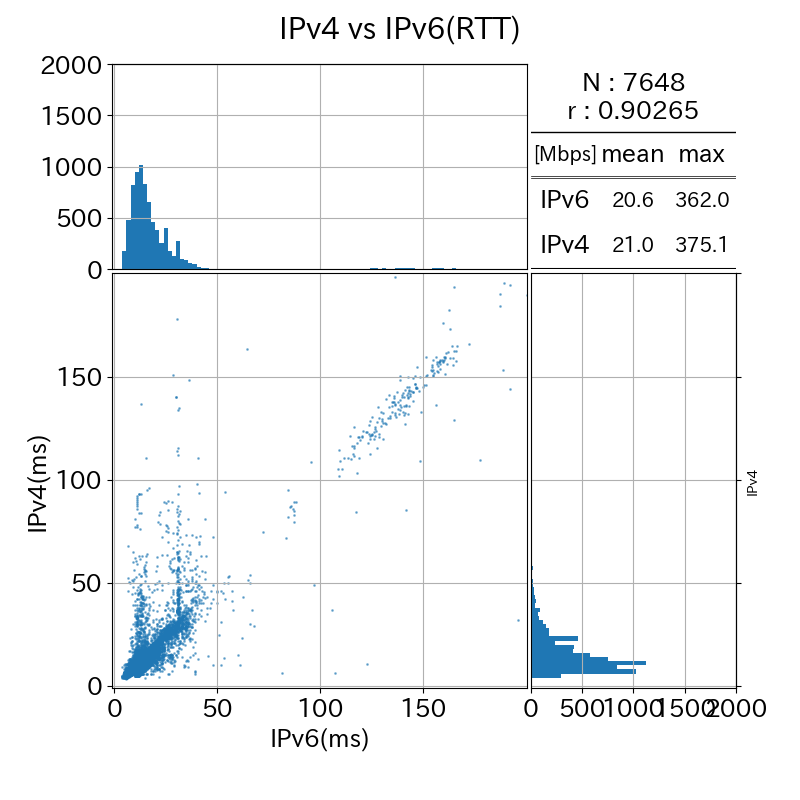
\includegraphics[width=0.85\textwidth]{fig/old_FTTH_rtt.png}
                    \subcaption{FTTHを使用した場合}
                    \label{old_FTTH_rtt}
                \end{subfigure}
                \begin{subfigure}[b]{\textwidth}
                    \centering
                    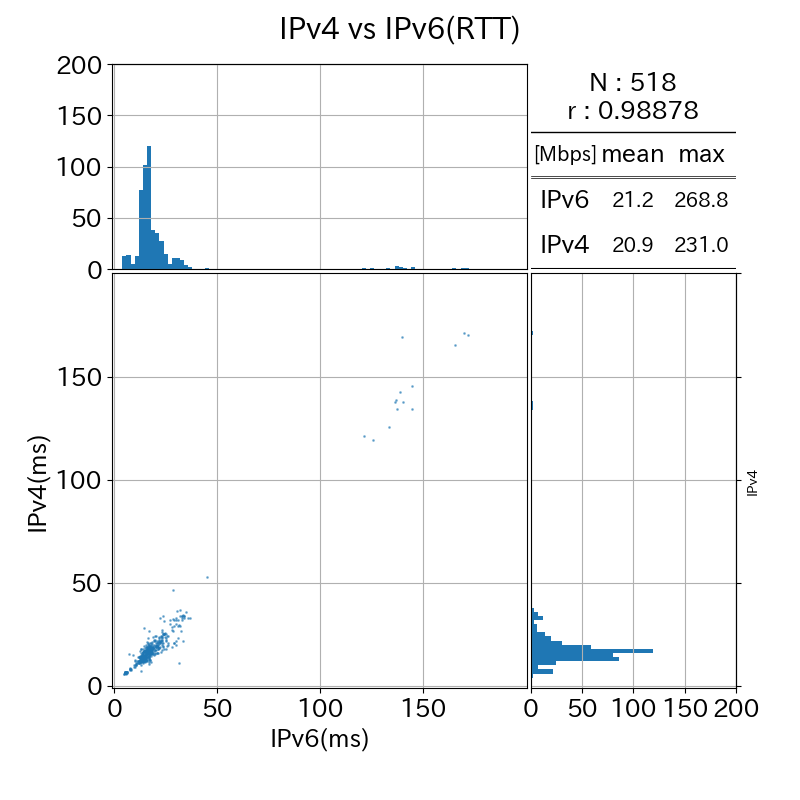
\includegraphics[width=0.85\textwidth]{fig/old_CATV_rtt.png}
                    \subcaption{CATVを使用した場合}
                    \label{old_CATV_rtt}
                \end{subfigure}
                \begin{subfigure}[b]{\textwidth}
                    \centering
                    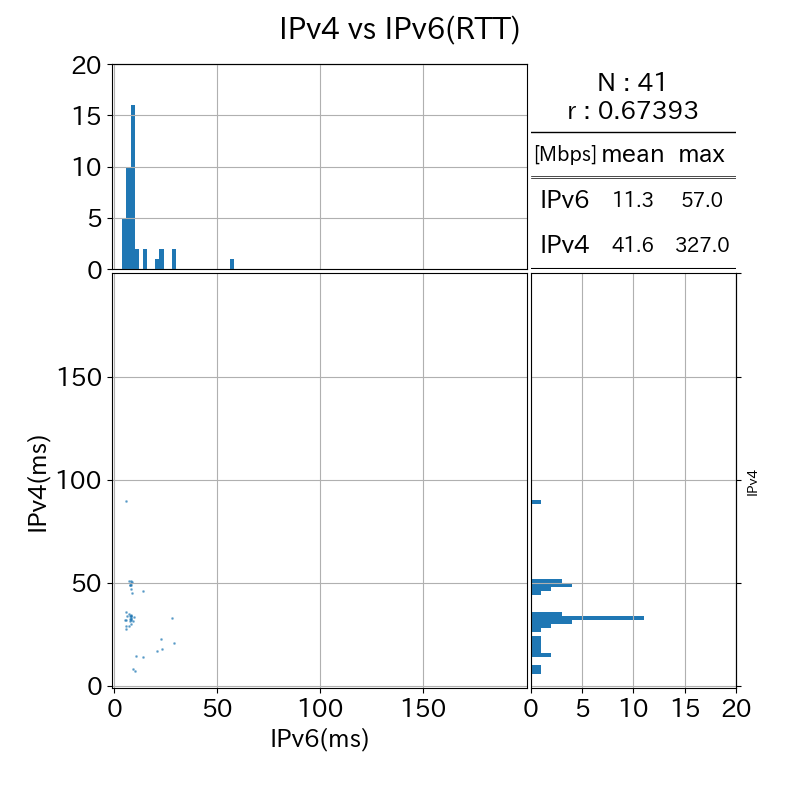
\includegraphics[width=0.85\textwidth]{fig/old_Mobile_rtt.png}
                    \subcaption{Mobileを使用した場合}
                    \label{old_Mobile_rtt}
                \end{subfigure}
            \caption{(1)のRTT}
            \label{fig:old_Line_rtt}
            \end{center}
        \end{minipage}
        \hfill
        \begin{minipage}[t]{0.48\textwidth}
            \begin{subfigure}[b]{\textwidth}
                \centering
                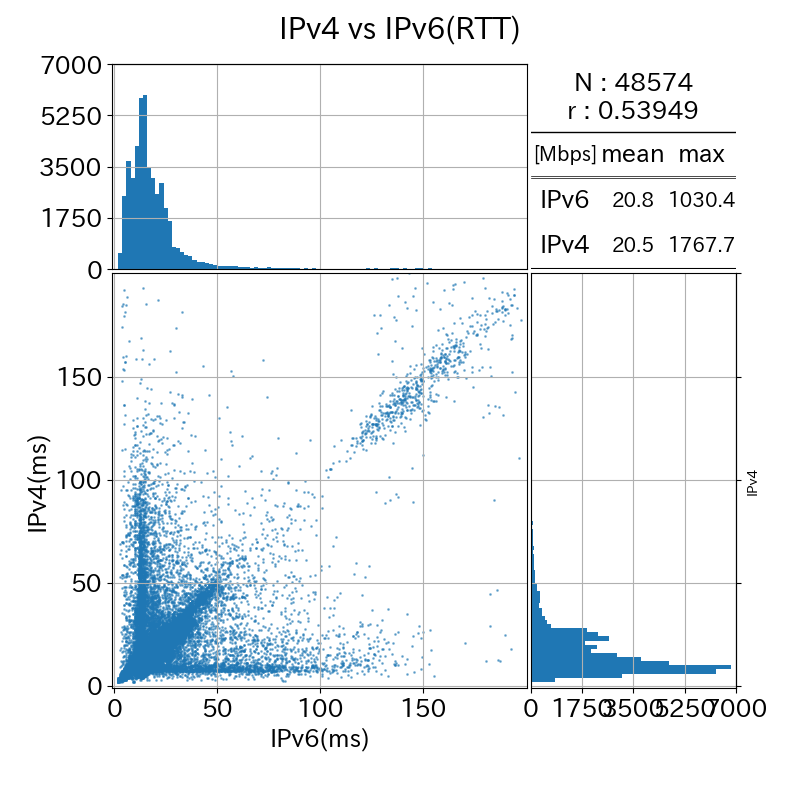
\includegraphics[width=0.85\textwidth]{fig/new_FTTH_rtt.png}
                \subcaption{FTTHを使用した場合}
                \label{new_FTTH_rtt}
            \end{subfigure}
            \begin{subfigure}[b]{\textwidth}
                \centering
                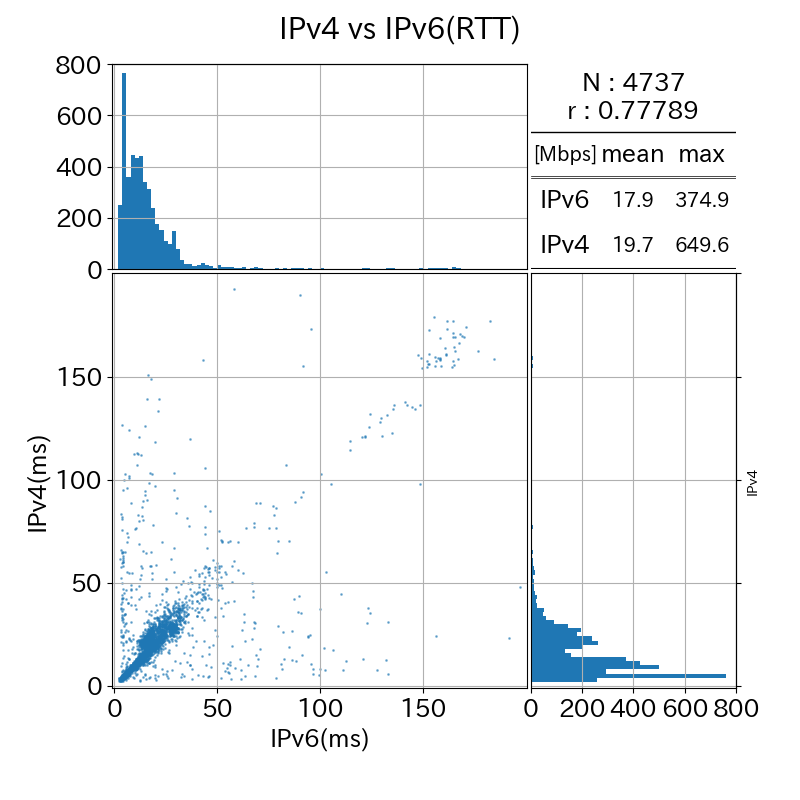
\includegraphics[width=0.85\textwidth]{fig/new_CATV_rtt.png}
                \subcaption{CATVを使用した場合}
                \label{new_CATV_rtt}
            \end{subfigure}
            \begin{subfigure}[b]{\textwidth}
                \centering
                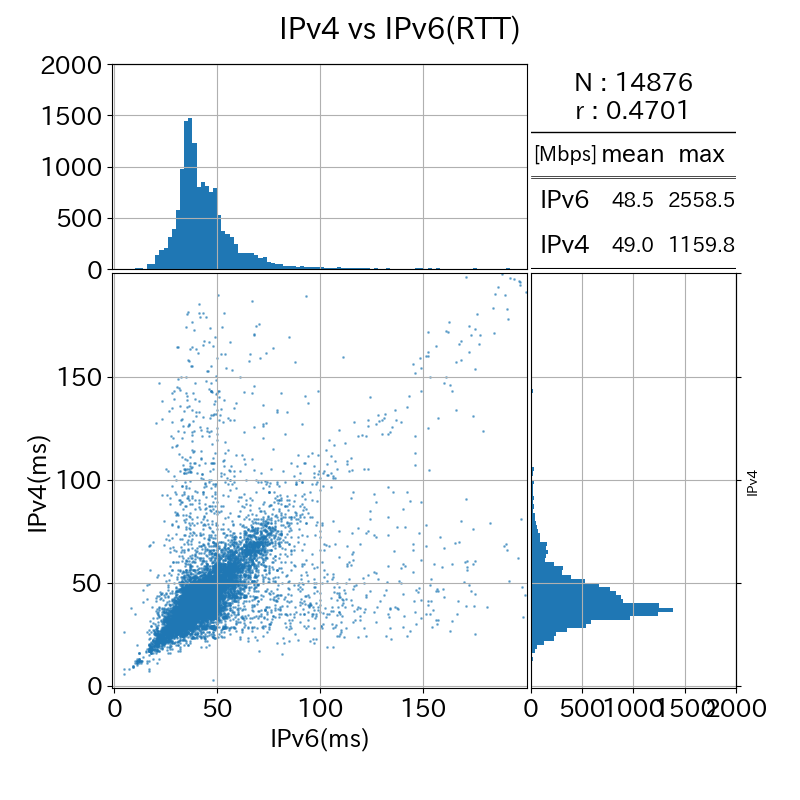
\includegraphics[width=0.85\textwidth]{fig/new_Mobile_rtt.png}
                \subcaption{Mobileを使用した場合}
                \label{new_Mobile_rtt}
            \end{subfigure}
            \caption{(2)のRTT}
            \label{fig:new_Line_rtt}
        \end{minipage}
    \end{center}
\end{figure}
\FloatBarrier
%\end{comment}

%\begin{comment}
\begin{figure}
    %\centering
    \begin{center}
        % 左側の図
        \begin{minipage}[t]{0.48\textwidth}
            \begin{subfigure}[b]{\textwidth}
                \centering
                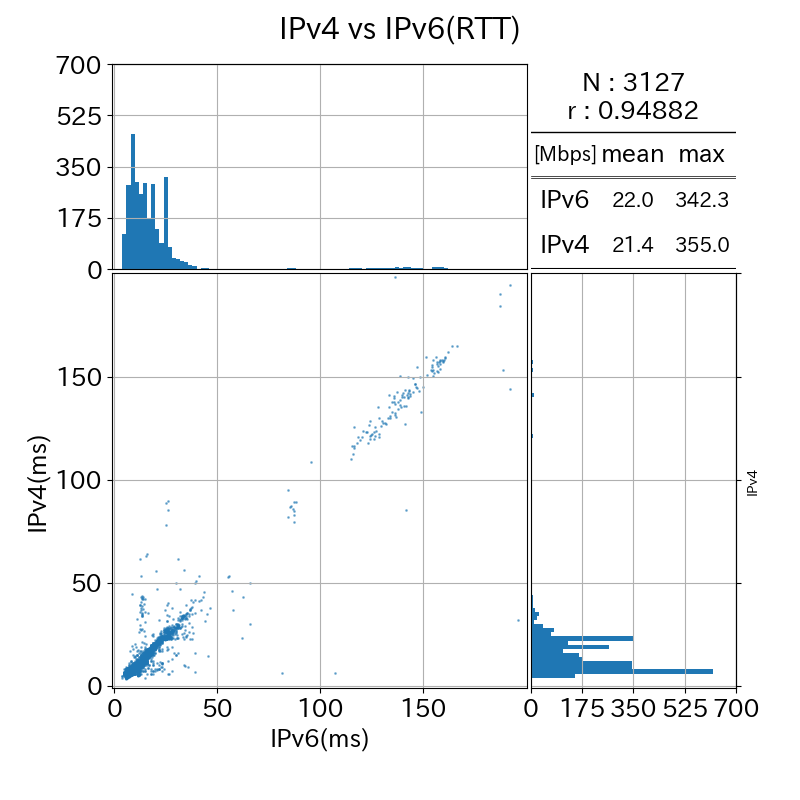
\includegraphics[width=0.85\textwidth]{fig/old_IPv4aaS_rtt.png}
                \subcaption{IPv4/IPv6でIPoEを使用した場合}
                \label{old_IPv4aaS_rtt}
            \end{subfigure}
            \begin{subfigure}[b]{\textwidth}
                \centering
                \includegraphics[width=0.85\textwidth]{fig/old_mix_rtt.png}
                \subcaption{IPv4はPPPoE,IPv6はIPoEを\\使用した場合}
                \label{old_mix_rtt}
            \end{subfigure}
            \begin{subfigure}[b]{\textwidth}
                \centering
                \includegraphics[width=0.85\textwidth]{fig/old_PPPoE_rtt.png}
                \subcaption{IPv4/IPv6でPPPoEを使用した場合}
                \label{old_PPPoE_rtt}
            \end{subfigure}
            \caption{(1)のRTT}
            \label{fig:old_connect_rtt}
        \end{minipage}
        \hfill
        \begin{minipage}[t]{0.48\textwidth}
            \begin{subfigure}[b]{\textwidth}
                \centering
                \includegraphics[width=0.85\textwidth]{fig/new_IPv4aaS_rtt.png}
                \subcaption{IPv4/IPv6でIPoEを使用した場合}
                \label{new_IPv4aaS_rtt}
            \end{subfigure}
            \begin{subfigure}[b]{\textwidth}
                \centering
                \includegraphics[width=0.85\textwidth]{fig/new_mix_rtt.png}
                \subcaption{IPv4はPPPoE,IPv6はIPoEを\\使用した場合}
                \label{new_mix_rtt}
            \end{subfigure}
            \begin{subfigure}[b]{\textwidth}
                \centering
                \includegraphics[width=0.85\textwidth]{fig/new_PPPoE_rtt.png}
                \subcaption{IPv4/IPv6でPPPoEを使用した場合}
                \label{new_PPPoE_rtt}
            \end{subfigure}
            \caption{(2)のRTT}
            \label{fig:new_connect_rtt}
        \end{minipage}
    \end{center}
\end{figure}
\FloatBarrier
%\end{comment}

%%%%%%%%%%%%%%%%%%%%%%%%%%%%%%%%%%%%%%%%%%%%%%%%%%%%%%%%%%%%%%%%%%%%%%%%%%
\section{調査のまとめ}
本章ではアクセス環境による通信品質への影響を調査した.スループットにはアクセス環境によって異なる振る舞いが見られた.ISP網内の通信環境や,アクセス網の種類の限界,インターネット接続方式の組み合わせの違いなどさまざまな要因でスループットに影響があるため,分析時には慎重な判断が必要である.CATVのように時期によって振る舞いが変化場合や,インターネット接続方式の違いのように他の要因も考えられる場合もあることから,引き続き調査をする必要があることがわかった.
一方,RTTについてはアクセス環境による振る舞いの違いはほとんど見られなかった.RTTはアクセス環境の種類よりも,地域による影響が大きいと予想される.先行研究\cite{nasu}では物理的距離だけでなくISP内のトポロジーやISP間の経路による影響が確認されている.これらの要因がスピードテストサイトの計測ログにも同様の傾向が見られるか調査するために,計測ログに付与する情報を増やし新たなアクセス環境を定義して調査する必要がある.

これらの結果から,スピードテストサイトの計測ログを使用して通信品質の分析をするとき,対象とアクセス環境のデータを抽出してから分析を行うことが重要であることがわかった.